\chapter{Regras Alternativas: A Customização do UNO}

Depois de analisar as estratégias para o jogo oficial (na sua variante 1121), podemos agora finalmente pensar em flexibilizar, customizar o UNO; \textbf{modificar} suas regras ou \textbf{inserir} novas, e considerar o \textbf{impacto estratégico} dessas modificações em \textbf{jogos normais}, com \textbf{apenas dois jogadores} ou com \textbf{parceiros}.

Além disso, considera-se também \textbf{como proceder} em casos em que a regra nova parece não se adaptar bem a certas regras oficiais --- ou \textbf{como ela funciona} em conjunto com \textbf{outras regras alternativas}.

Mesmo essas regras (muitas delas) possuem muitas flexibilizações internas e escolhas a serem feitas; Considerei, dentro do possível, todas essas diferenças e expliquei por que escolhi um modo de implementar essas regras, e não outro. Se o motivo não for razoável o suficiente, as opções ficam em aberto (e deixo isso claro no final de cada regra).

Todas as regras contêm \textit{siglas}; isso ajuda depois a definir o seu tipo preferido de jogo e então criar um código para lembrar de todas as regras que ele encerra.

Você já deve ter tido contato com muitas regras, mas provavelmente não com todas. Divirta-se!

\section{Regras que Modificam o Objetivo do Jogo}

Essas regras modificam o Objetivo do Jogo. Lembre-se, do \textit{jogo}, não da \textit{partida}; a diversão ainda está em livrar-se das cartas na mão, mas o que você faz \emph{assim} que isso acontece pode ser modificado.

\subsection{Número de Pontos}

Uma observação inicial a ser feita é que uma das coisas mais usualmente flexibilizadas é o número de pontos no UNO a serem alcançados para que um jogador possa ser considerado vencedor: os 500 geralmente se tornam menos caso os jogadores não queiram que uma partida torne-se muito longa.

Mesmo sem adotar uma das regras que modificam o objetivo do jogo, tenha em mente que esse número pode sempre ser flexibilizado para as suas vontades (princípio que vale também para, por exemplo, a Regra dos Pontos Reversos --- ver abaixo, na página \pageref{pontosreversos}). 

\subsection{Regra do Torneio de Vitórias [TV]}

Ao invés de acumular 500 pontos, você pode abandonar de vez a ideia de pontos e jogar apenas por número de vitórias; em um jogo com várias pessoas, o primeiro a vencer \textit{x} vezes é o campeão; em um jogo de duas pessoas, uma melhor de 3, 5 ou 7\footnote{Uma ``melhor de três'' é uma expressão utilizada para definir uma sequência de três jogos em que aquele entre dois adversários que vence mais partidas é o vencedor. É particularmente interessante pois se há apenas dois jogadores e três partidas, aquele que vence duas é automaticamente o campeão, não precisando que uma terceira partida seja jogada. Em uma ``melhor de cinco'', por exemplo, aquele que vence três partidas é o campeão (a mesma lógica de um jogo de vôlei, por exemplo). Essa ideia, contudo, não serve para jogos com mais de dois jogadores.} pode ser o esquema usado. De uma forma ou de outra, a contagem de pontos sequer é feita.

\subsubsection{Consequências}

Esta regra, embora possa parecer inócua, possui profundas consequências na dinâmica de jogo e em aspectos externos do jogo. Vamos começar por este último caso: no Torneio de Vitórias, os pontos não são contados ao final da partida. Isso pode levar a partidas mais rápidas. Por outro lado, as diferenças estratégicas provocadas por essa regra, como veremos adiante, pode acabar compensando esse tempo ao tornar mais longo o jogo.

No quesito estratégia, temos que tudo que importa é \textit{vencer}; nesse caso, muitas das estratégias estudadas deixam de trazer consigo qualquer espécie de \textbf{risco}. É importante que se entenda isso: se um jogador perde, não importa mais com que cartas foi pego na mão; isso é irrelevante agora. A carta zero, por exemplo, deixa de ser uma carta valorizada como tática defensiva em momentos de tensão, e o Curinga Surpresa é uma estratégia que passa a ser empregada com uma frequência absurdamente maior. Esse tipo de modificação na dinâmica do jogo ocorre em qualquer tipo de jogo UNO: individual, com dois jogadores ou em duplas.

Como dito anteriormente, isso também possui impacto no tempo de jogo: sem a pressa para livrar-se das cartas e com a paciência para explorar todos os tipos de estratégia que envolvem \textit{manter} as cartas na mão, o jogo pode vir a demorar um pouco mais --- fazendo com que, no final das contas, um jogo pautado por esta regra não seja, afinal de contas, mais rápido.

\subsubsection{Variações}

Não só as vitórias podem ser contadas, mas a exemplo da Regra dos Pontos Reversos (a ser vista logo abaixo), as derrotas podem ser a base da contagem de pontos: todos os jogadores podem começar com um número \emph{x} de pontos e ir perdendo um ponto a cada derrota. 

\subsubsection{Indicado}

para pessoas que queiram experimentar mais livremente com possibilidades estratégicas, sem sentir a pressão da pontuação, ou para pessoas que queiram simplesmente jogar sem ter que contar pontos.

\subsection{Regra dos Pontos Reversos [PR]}

\label{pontosreversos}

Ao invés de acumular 500 pontos, todos os jogadores \textit{começam} com 500 pontos e, ao longo do jogo, vão perdendo-os com base nas cartas que permanecem em suas mãos após a vitória de algum dos jogadores.

\subsubsection{Consequências}

Esta regra pode, novamente, parecer não fazer muita diferença, mas na verdade faz: em um jogo onde o objetivo é acumular pontos a partir dos pontos remanescentes nas mãos dos perdedores, um objetivo secundário do jogo torna-se, muitas vezes, fazer com que os jogadores \textit{comprem} cartas e \textit{mantenham} essas cartas na mão.

Ao mesmo tempo em que o fator da continuidade tem sido apontado ao longo do livro como a estratégia mais relevante para a vitória de uma partida e, consequentemente, do jogo, o UNO é um jogo de flexibilidade em que várias táticas podem ser seguidas (por vezes simultaneamente), com variados graus de sucesso. Para ganhar mais rapidamente, fazer com que os jogadores comprem cartas não deixa de ser importante.

Em um jogo onde esses pontos remanescentes não se combinam para formar a pontuação de alguém, mas apenas são subtraídos do total individual, o importante é tentar ganhar com cautela, para não perder muitos pontos caso alguém seja mais rápido. Enquanto o jogo normal favorece o ataque e artimanhas que vão na contramão da continuidade apenas em nome da ofensividade, este tipo de jogo acaba incentivando uma atitude mais defensiva, em que tudo que é feito o é exacerbando a importância de se livrar de cartas de ação para evitar ter muito prejuízo com a vitória alheia.

Além disso, essa dinâmica de jogo faz com que o jogo fique mais longo: quando alguém perde seus 500 pontos, sai do jogo, mais os outros continuam a jogar até que reste apenas um jogador que ainda possui pontos. Dessa forma, o jogo demora mais para chegar ao fim (embora não o mesmo tempo para todos os envolvidos).

\subsubsection{Indicado}

para pessoas que prefiram um jogo em que apenas os mais prudentes (não necessariamente os \emph{melhores} jogadores) vão resistindo ao tempo, ajudando a moldar uma espécie de ``partida final''.

\subsection{Regra da Morte Súbita [MS]}

Nesse jogo, não só ficar com nenhuma carta na mão é importante, mas também continuar a jogar. Esta é, \emph{par excellence}, a variação da continuidade: o jogador que for obrigado a comprar uma carta (exceto por meio de cartas Comprar Duas / Comprar Quatro, além de punições) é eliminado do jogo, e os outros continuam até sobrar apenas um ou alguém descartar todas as cartas da mão. Note-se que por ``ser obrigado a comprar uma carta'' deve-se entender que o próprio ato de compra leva à eliminação --- o jogador que não puder jogar com as cartas que tem à mão, quando for sua vez, é eliminado.

\subsubsection{Consequências}

Em primeiro lugar, as partidas se tornam mais rápidas, pois quem é obrigado a comprar não permanece jogando. Em segundo lugar, nenhum outro aspecto e impulso do jogo se torna mais primordial do que a continuidade: fazer o outro comprar não é mais relevante, o que é importante é planejar o jogo de modo a aumentar as suas chances de \emph{continuar jogando}. É um jogo de dinâmica rápida e, por isso mesmo, mais tenso que os outros.

\subsubsection{Variações}

\begin{description}
\item[Morte Súbita Sem Proteção (MS1)]{Qualquer jogador, desde o princípio do jogo, está sob o risco de ser eliminado.}
\item[Morte Súbita Com Proteção (MS2)]{Apenas depois de um número \textit{x} de rodadas a Morte Súbita começa a valer. Número sugerido: duas rodadas.}
\item[Morte Súbita Com Trava (MS3)]{Apenas após algum evento do jogo a Morte Súbita começa a valer; o primeiro Curinga a ser jogado, a primeira carta de um determinado número a ser jogada, a quinta carta de ação a ser jogada, etc.}
\end{description}

\subsubsection{Possíveis Contradições e Conexões}

\begin{description}
\item[Pontuação]{Para fazer a pontuação, vários métodos anteriormente vistos podem ser usados: quem for eliminado pode ter suas cartas revertidas como pontos para o vencedor (que ainda está por ser decidido), ou pode perder pontos (se o esquema de pontos reversos for utilizado), etc.}
\item[Regra do Passe ou do Inferno]{Se esta regra for aplicada em conjunto com qualquer variação da Regra do Passe ou com a Regra do Inferno, não ter uma carta Comprar Duas, Comprar Quatro ou carta de ataque que possa ser jogada garante uma eliminação.}
\item[Regra do Final Limpo]{Caso a regra do Final Limpo seja aplicada, caso a pessoa possua como última carta uma carta que ela não pode jogar, este jogador deve ser eliminado.}
\item[Regra do Corte]{Se aplicada conjuntamente com a regra do corte, pode gerar algumas dúvidas: supondo que o jogador A vá jogar, mas não possa (\emph{i.e} será eliminado), mas antes que \emph{declare} que será eliminado, outro jogador corta sua vez --- neste caso, o jogador A não é eliminado. Se ele já tiver declarado que será eliminado, o jogador B é quem será cortado, e o jogador A terá sido eliminado.}
\item[Regras da Paz]{As regras de paz impedem que cartas de ação sejam jogadas durante períodos específicos de tempo. Assim sendo, se não for possível jogar uma carta de ação num dado momento e o jogador, posto isso, \emph{não conseguir} jogar \emph{carta alguma}, a lógica permanece: o jogador é eliminado.}
\item[Regra do Descarte Duplo]{Se jogada em conjunto com a regra do Descarte Duplo: se o jogador A não tiver o que jogar e, para não ser eliminado, mentir e for pego mentindo, é eliminado (e os outros jogadores agem de acordo com os mecanismos da Regra do Descarte Duplo. Se jogar de forma oculta, o acusarem de mentira, mas sua jogada for legítima, novamente os mecanismos do Descarte Duplo se aplicam).}
\item[Outras Punições]{Sempre que um jogador for obrigado a comprar uma carta devido a uma \emph{punição} (como, por exemplo, a Regra do Silêncio ou a do Monte) isto não o elimina; um jogador é apenas eliminado se não puder jogar nenhuma carta que estiver em sua mão no momento --- por exemplo, se com a Regra de Chukcki aplicada um jogador não puder jogar uma carta (ou uma combinação de cartas) que altere a cor da pilha de descarte, ele será eliminado.}
\end{description}

\subsubsection{Indicado}

para quem tem pouco tempo disponível para jogar ou para quem prefira um jogo mais imprevisível.

\section{Regras que Modificam a Dinâmica de Jogo}

Essas regras modificam o modo como o jogo é jogado, partindo de características como o número de cartas com que uma pessoa começa o jogo, passando por regras que determinam aquilo que pode ser descartado, e indo até regras que restringem o comportamento de um jogador.

\subsection{Regra do Final Limpo [FL]}

Os jogadores podem apenas vencer o jogo com cartas numéricas, cartas Pular e Inverter. Curingas e cartas que obriguem os jogadores a comprar não podem, portanto, ser usadas para vencer.

\subsubsection{Consequências}

A consequência mais imediata é o fim da estratégia do Curinga Surpresa (já discutido anteriormente), uma vez que você não pode guardar mais o Curinga como última carta.

Esta regra costuma ser mais impactante, contudo, quando jogada em conjunção com variações da Regra do Passe (ver mais adiante, página \pageref{regradopasse}). É uma estratégia comum (pois muito eficaz) guardar um Comprar Duas ou Comprar Quatro como última carta (neste último caso, é mesmo um Curinga Surpresa, mas com outras vantagens) pois caso alguém tente fazê-lo comprar cartas na última rodada, você pode se defender. Com a Regra do Final Limpo, ganhar o jogo desse jeito (que alguns podem considerar chato por ser até muito fácil) torna-se impossível.

\subsubsection{Variações}

Pode-se estipular que só se pode ganhar o jogo com cartas numéricas; ou que não se pode ganhar o jogo com Curingas (mas cartas de Compra são permitidas, uma regra que faz sentido se o grupo não joga com Regras do Passe).

\subsubsection{Possíveis Contradições e Conexões}

\begin{description}
\item[Impossibilidade]{À exemplo da Primeira Regra da Paz (ver adiante na página \pageref{primeirapaz}), essa regra não estipula punições, e sim determina a \emph{impossibilidade} de jogar certas cartas para ganhar o jogo.}
\item[Regra do Passe e do Inferno]{Se jogada em conjunto com a Regra do Passe ou a Regra do Inferno, significa que se um jogador A joga uma carta Comprar Duas e o jogador B estiver UNO (sua carta sendo um outro Comprar Duas ou uma carta que poderia ser jogada, mas não pode por causa do Final Limpo), ele não poderá usar essa carta para vencer o jogo; deverá comprar duas cartas.}
\item[Desafio Polivalente]{Se jogada em conjunto com a Regra do Desafio Polivalente, a lógica é a seguinte: Se um jogador A não pode descartar o Curinga (por exemplo) pois é a sua última carta, e precisa comprar, se alguém o desafia, deve comprar quatro cartas, pois ele de fato precisava comprar.}
\item[Regra do Descarte Duplo]{Se jogada em conjunto com a regra do Descarte Duplo: se o jogador A tiver como última carta uma carta que não possa ser jogada, ele pode tentar ganhar o jogo mentindo. No caso de ser descoberto, os mecanismos da Regra do Descarte Duplo se aplicam. Se não tiver mentido, os mesmos mecanismos se aplicam.}
\item[Regra do Corte]{Se um jogador A possui como última carta uma carta que não pode ser jogada para vencer, o jogador também não pode vencer com esta carta ao fazer um corte. Ele não pode jogá-la, seja numa jogada normal, seja num corte.}
\item[Regra do Descarte Rápido e Duplicatas]{Como os jogadores não podem \emph{vencer} com as cartas que forem combinadas no começo do jogo, eles não podem fazê-lo, mesmo se não estiverem UNO. Por exemplo: o jogador A não pode vencer com um Curinga, e também não pode vencer jogando dois curingas de uma vez só (sem ficar UNO).}
\item[Cartas com funções]{Se a partir de qualquer regra alternativa uma carta comum ganhar a função de fazer algum jogador comprar cartas, esta carta não pode ser usada para vencer o jogo.}
\end{description}

\subsubsection{Indicado}

para quem acredita que assim o jogo se torna mais difícil e taticamente complexo, uma vez que a estratégia do Curinga Surpresa pode ser (dependendo de algumas combinações de regras específicas) muito fácil de ser realizada.

\subsection{Regra do Flash UNO [FU]}

Ao invés das oficiais 7 cartas, todos os jogadores começam o jogo com 4 cartas.

\subsubsection{Consequências}

Com menos cartas iniciais, a duração de cada partida tende a ser menor. Em compensação, as estratégias tendem a ser mal formuladas ou não-formuladas \emph{at all}, incluindo certa confusão, desde o início, entre que papel se deve exercer no jogo (o de gerenciador ou de fugitivo do gerenciamento alheio). Dessa forma, é um jogo em que a estratégia é exercida de forma limitada, e pode apenas vir a exercer um papel mais proeminente na decisão da partida se todos os jogadores acabarem por comprar mais cartas.	

\subsubsection{Variações}

Na verdade o número de 4 cartas é uma arbitrariedade; poderia ser qualquer número de 6 para baixo (com o 6 não fazendo muita diferença, e o 2 fazendo uma diferença verdadeiramente \emph{excruciante} em termos de importância tática).

\subsubsection{Indicado}

para quem tem pouco tempo disponível para jogar; para aqueles que desejam um jogo mais rápido.

\subsection{Regra do Battlefield UNO [BU]}

O Battlefield UNO é o inverso do Flash UNO: Ao invés das oficiais 7 cartas, todos os jogadores iniciam o jogo com 9 cartas.

\subsubsection{Consequências}

As possibilidades de gerenciamento são maiores e o jogo geralmente torna-se mais longo e intrincado.

\subsubsection{Variações}

Assim como no Flash UNO, o número 9 é arbitrário: pode ser qualquer número de 8 para cima.

\subsubsection{Indicado}

para quem deseja um jogo em que muitas reviravoltas e tramas estratégicas possam ocorrer. Indicado também especialmente para jogos com apenas dois jogadores, em que um número de apenas 7 cartas pode tornar o jogo rápido demais.

\subsection{Regra do Corte [C]}

\label{regradocorte}

Uma das regras alternativas mais populares, a Regra do Corte estipula que cartas \emph{idênticas} (iguais em número/símbolo e cor) possam ser jogadas consecutivamente por dois jogadores que não estão necessariamente na ordem normal do jogo. Na prática, se pensarmos em um jogo-exemplo entre os jogadores A, B, C, D, E e F (que jogam nesta ordem) poderemos ter uma ideia mais precisa do sentido da regra:

O jogador A joga um 5 Verde na pilha de descarte. O jogador B prepara-se para jogar, mas uma vez que tenha demorado muito, o jogador D (que não é o próximo a jogar) joga uma carta idêntica (outro 5 Verde, portanto) na pilha de descarte. Essa jogada é chamada de ``corte'', pois corta a ordem natural do jogo. Depois do corte, o jogo prossegue a partir do ponto de corte; o jogador B, cortado, não joga, e nem o jogador C: agora o jogador E continua, e depois dele o jogador F, e então o jogador A, e apenas aí o jogador B poderá jogar novamente.

\begin{figure}[!h]
\centering
\fbox{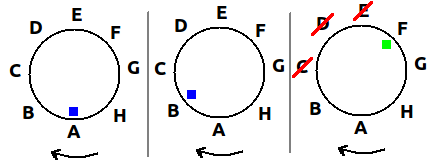
\includegraphics[scale=0.7]{fig8.png}}
\caption{O jogador A joga, então é a vez do jogador B, mas antes que o jogador C jogue, o jogador F joga uma carta idêntica à que está na pilha de descarte. Os jogadores C, D e E perdem a vez (\emph{são cortados}), e então G continua o jogo.}
\end{figure}

Outros exemplos, utilizando-se dos mesmos jogadores: o jogador C joga um 7 Vermelho. O jogador A poderia cortar o jogo com seu 7 Vermelho à mão, mas o jogador D foi mais rápido e continuou o jogo; agora já não há mais possibilidade de corte. O corte só pode acontecer enquanto o próximo jogador não joga seu turno; lembre-se que comprar uma carta conta como jogar um turno. Além disso, se o jogador E joga um 2 Azul e o jogador F também possui um 2 Azul, ele pode jogá-la normalmente; é como um corte, porém já que o jogador que corta é o mesmo que normalmente jogaria, não há diferença alguma.

\subsubsection{Consequências}

O jogo torna-se muito mais tenso e animado, uma vez que \emph{todos os jogadores devem prestar atenção ao jogo o tempo todo}. Isso ocorre porque agora qualquer jogada é oportuna e, ao mesmo tempo, na própria vez, você deve jogar rapidamente para evitar que outro corte sua vez.

O pensamento estratégico de longo prazo, contudo, é um tanto prejudicado nesse jogo, uma vez que existe uma pressão para que as jogadas sejam feitas rapidamente, sob o risco de perder a vez.

\subsubsection{Possíveis Contradições e Conexões}

\begin{description}
\item[Momentos de Corte]{O corte pode ser feito por qualquer jogador, a qualquer momento do jogo em que se pode normalmente jogar. Um jogador pode ``ficar UNO'' através de um corte, e pode também ganhar o jogo a partir de um corte. Um jogador não pode cortar a si mesmo, contudo, quando uma carta de compra tiver sido jogada (para se livrar da punição de comprar o número estipulado de cartas).}
\item[Compra]{Se o jogador A jogar um 5 Vermelho e o jogador B precisar comprar uma carta, o jogador B pode ser cortado antes de comprar e depois de comprar. Neste último caso, quem está sendo cortado, na verdade, é o jogador C; se o jogador B comprar e puder \emph{jogar aquilo que comprou}, ninguém pode cortá-lo.}
\item[Jogadas Equivocadas]{Da mesma forma que jogadas equivocadas devem ser punidas com a compra de duas cartas, cortes equivocados devem ser penalizados da mesma maneira.}
\item[Punições]{Um jogador não pode cortar a si mesmo quando é sua vez de receber uma punição, como dito acima; dessa forma, se o jogador A joga uma carta Comprar Duas Verde, o jogador B não pode cortar a si mesmo para que o jogador C compre quatro cartas. Entende-se, contudo, que algum \emph{outro jogador}, que não o B, possa cortar o jogo, porque quem ele cortará, na verdade, será o jogador C (de modo que o jogador B ainda precisa comprar as duas cartas).\footnote{A maioria das pessoas, contudo, joga com alguma variação da regra do passe, e vai compreender melhor como o corte se aplica ao ler o ítem logo abaixo deste, o ``Punições Acumuladas''}.}
\item[Punições Acumuladas]{Quem preferir jogar em conjunto com qualquer variação da Regra do Passe ou com a Regra do Inferno deverá jogar de acordo com a seguinte dinâmica: se o jogador A joga uma carta Comprar Dois Amarela, qualquer outro jogador pode cortar \emph{o jogador B}, então se o jogador C joga a outra carta Comprar Dois Amarela, o jogador \textbf{D} deve comprar quatro cartas. Contudo, há ainda outra opção: deixar que o jogador B compre as duas cartas e então cortar o jogador C, antes que ele jogue ou compre uma carta. A coisa fica ainda mais curiosa e interessante com as cartas Curinga Comprar Quatro, uma vez que se uma for jogada, três cortes podem ser feitos, e alguém pode ser obrigado a comprar 16 cartas.}
\item[Cartas de Ação com Cortes]{Quando cortes forem feitos envolvendo cartas de ação, algumas regras específicas se aplicam:
\begin{description}
\item[Carta Pular]{Se o jogador A joga uma carta Pular (fazendo com que o jogador B não jogue), qualquer corte feito sobre essa carta anula o efeito da carta cortada, e agora apenas o efeito novo sobra. Dessa forma, num jogo entre A, B, C e D, se o jogador A joga uma carta pular e for cortado pelo jogador C, quem na verdade é pulado é o jogador D, e o jogador A deve, portanto, jogar novamente.}
\item[Carta Inverter]{Dessa vez, de certa forma o corte considera o efeito anterior: se os jogadores A, B, C, D e E jogam nesta ordem, o jogador A joga uma carta Inverter e faz com que o jogador E seja o próximo. Antes que o jogador E jogue, contudo, o jogador B corta: se, então, a ordem do jogo acabara de se tornar A--E--D--C--B, a ordem volta a ser A--B--C--D--E, e como começa agora do jogador B, o jogador C é o próximo a jogar.}
\item[Curinga]{Se um Curinga for cortado, a escolha de cor anterior é ignorada e o jogador que fez o corte escolhe a cor. Como de praxe, o jogo prossegue do jogador que cortou, com a cor escolhida agora por ele.\footnote{Para entender melhor sobre a dinâmica do Curinga Comprar Mais Quatro, contudo, leia o ítem ``Punições''.}}
\end{description}
}
\item[Duas Pessoas]{Com UNO jogado entre duas pessoas, o efeito desta regra é diminuto, mas um pouco significativo; em um jogo oficial 1121, funciona como uma espécie de Regra das Duplicatas (o jogador que jogou uma carta pode jogar outra idêntica ao mesmo tempo). Além disso, como em um jogo entre duas pessoas uma carta Pular significa que o mesmo jogador joga novamente, cortar esta carta Pular significa impedir essa jogada.}
\item[Parcerias]{Em um jogo de parcerias, a regra do Corte costuma ser pouco benéfica. Imaginando um jogo exemplo entre os jogadores A, B, C e D, duplas A e C, B e D, e a ordem do jogo é ABCD, vamos acompanhar o ponto de vista do jogador A: cortar durante a vez do jogador B significa apenas jogar duas vezes. Bom, mas é, como foi discutido no ítem acima, como a Regra das Duplicatas. Cortar o próprio parceiro é péssimo: o jogador A jogaria novamente, mas o jogador B também. Cortar o jogador D faria com que o jogador A e o C jogassem novamente, mas também o C. O que se demonstra é que quanto maior o número de pessoas, mais efetivo o Corte pode ser. Em pequenos números e, em especial, em Parcerias, a regra não surte tanto efeito positivo para quem a aplica.}
\item[Chukcki]{Ao jogar em conjunto com a Regra do Chukcki, ocorre o seguinte: considere os jogadores A, B e C (que estão jogando entre mais jogadores). O jogador A joga uma carta numérica, e o jogador B joga uma carta de mesmo valor numérico. O jogador C deve, através de quaisquer mecanismos apropriados, mudar a cor da pilha de descarte. As jogadas do jogador A e B podem ser originadas de um Corte. Contudo, \emph{não considerando outras regras}\footnote{A Regra do Descarte Rápido tornaria um Corte possível para o jogador C, por exemplo.}, uma vez que o corte trata de cartas \emph{idênticas}, ninguém vai conseguir mudar a cor da pilha de descarte com um corte.}
\item[Duplo Descarte]{Ao jogar com a regra do Duplo Descarte, apenas as cartas \emph{declaradas} valem: não se pode cortar uma carta que tenha sido omitida (mesmo que depois se descubra qual carta é) e não se pode cortar de forma ``omitida''.}
\end{description}

\subsubsection{Indicado} 

para jogos com \emph{muitos jogadores}, em que quando um joga, as pessoas do lado mais distante da mesa, que vão demorar para jogar novamente, não costumam prestar atenção ao jogo. Bom também para quem deseja um jogo mais imprevisível e complexo. Por outro lado, às vezes a tensão e a pressa ao jogar podem comprometer um estilo de jogo mais bem pensado, estratégico.

\subsection{Regra do Descarte Rápido [DR]}

\label{descarterapido}

Outra regra relativamente comum, a Regra do Descarte Rápido determina que cartas de mesmo número/símbolo possam ser jogadas na mesma rodada por um mesmo jogador. Dessa forma, o jogador A pode jogar três cartas 5 (uma verde, uma vermelha e uma azul), o jogador B pode jogar duas cartas (um 6 Azul e um 6 Verde), o jogador C pode jogar 4 cartas (Um 7 Verde, outro 7 Verde, um 7 Azul e um 7 Amarelo), e aí por diante. A única exigência para que uma carta possa ser jogada em cima de outra é que o número e/ou símbolo seja correspondente.

\begin{figure}[!h]
\centering
\fbox{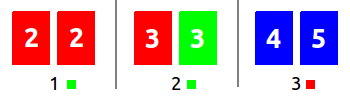
\includegraphics[scale=1]{fig9.png}}
\caption{A Regra do Descarte Rápido se aplica à situação 1 e à situação 2, por serem duas cartas de mesmo número/símbolo. Entretanto, \textbf{não} se aplica à situação 3, uma vez que apenas a cor é a mesma.}
\end{figure}

\subsubsection{Consequências}

Adiciona-se ao jogo uma dinâmica nova em que os jogadores não apenas ficam para trás por não terem cartas para jogar, mas também avançam, tornam-se mais rápidos que outros, por conseguirem se livrar de duas ou mais cartas em uma mesma rodada. Isso altera estratégias e insere um elemento de surpresa a mais no jogo, o que, por sua vez, torna o pensamento tático mais conveniente. 

\subsubsection{Possíveis Contradições e Conexões}

\begin{description}
\item[Diferenças]{Cartas Comprar Quatro não podem ser jogadas juntamente com cartas 4; cartas Comprar Duas não podem ser jogadas com cartas 2.}
\item[Acúmulo]{Cartas Comprar Quatro podem ser jogadas juntamente com outras Comprar Quatro (fazendo com que o próximo jogador obrigatoriamente compre o número acumulado de cartas. O mesmo vale para cartas Comprar Duas.}
\item[Ordem das Cartas]{No descarte rápido, é como se você jogasse a carta apropriada de acordo com a carta na pilha de descarte, e então adicionasse cartas de números ou símbolos iguais \textbf{acima} da carta apropriada. Dessa forma, se há um 3 Amarelo na pilha de descarte, e você pretende jogar, ao mesmo tempo, um 9 Azul, um 9 Amarelo e um 9 Vermelho, o 9 Amarelo deve ser jogado primeiro e, depois dele, você pode escolher a ordem em que quer deixar os outros 9s da jogada (primeiro o azul e depois o vermelho, ou o contrário).}
\item[Momento de Acúmulo e UNO]{As cartas podem ser jogadas de forma agrupada em qualquer momento em que uma única pode ser jogada normalmente. Dessa forma, uma pessoa pode ``ficar UNO'' ao jogar duas cartas ao mesmo tempo (tendo três cartas na mão e, após o descarte, tendo apenas uma), e uma pessoa pode vencer o jogo sem precisar se declarar UNO ao jogar suas duas últimas cartas de forma conjunta. Isso cunha um novo tipo de estratégia, similar ao Curinga Surpresa, conhecida como o \textbf{Grupo Surpresa} (ver abaixo, página \pageref{gruposurpresa}).}
\item[Vez]{Se um jogador for jogar várias cartas ao mesmo tempo, deve fazê-lo de uma vez só, ao mesmo tempo. Se não o fizer, deve declarar em tom suficientemente alto que sua jogada ainda não acabou e que ele ainda tem mais cartas a descartar\footnote{Especialmente em jogos em que a Regra do Passe é aplicada, alguns jogadores podem ter dificuldade para organizar na mão um grande número de cartas, o que leva a problemas pra jogar várias cartas de uma vez só rapidamente.}; se o próximo jogador na ordem do jogo já tiver comprado uma carta ou jogado uma carta (\emph{i.e} iniciado sua vez), o jogador anterior não poderá jogar mais cartas.}
\item[Cartas de Ação em Conjunto]{Quando cartas de ação forem jogadas em conjunto, algumas regras específicas se aplicam:
\begin{description}
\item[Carta Pular]{Se duas cartas Pular forem jogadas, dois jogadores são pulados; se três cartas forem jogadas, três são pulados, e assim por diante. Em um jogo com $n$ jogadores, se $n - 1$ cartas Pular forem jogadas, o próprio jogador que as jogou joga novamente. Se qualquer número de cartas de $n$ para cima for jogado, o próprio jogador é ignorado e apenas os adversários contam na contagem de ``pulos'' até a verificação de quem é o próximo a jogar (exemplo: num jogo entre A, B e C o jogador A jogou quatro cartas Pular; pulou o B, o C, depois o B novamente e enfim o C novamente, de forma que o B é o próximo a jogar.)\footnote{Cuidado como o jogo em duplas: estratégias derivadas do Isolamento exigem que uma carta Pular seja jogada de cada vez}.}
\item[Carta Inverter]{Se um número par de cartas Inverter for jogado em conjunto, então a ordem do jogo não se altera. Se um número ímpar for jogado, a ordem do jogo se altera.}
\item[Curinga]{Se vários curingas forem jogados, contam como um: o jogador que os jogou escolhe uma cor e o jogo prossegue normalmente.}
\item[Dedução]{Essa regra (e a das Duplicatas, adiante), permite uma dedução de relevância menor, mas que, combinada a outras informações e circunstâncias, pode ser útil: se um jogador tem duas cartas na mão e joga apenas uma, é porque a carta que permaneceu não é do mesmo número ou símbolo. No caso da regra das duplicatas, só significa que a carta não é idêntica, o que é de ainda menor utilidade, mas é um raciocínio que vale à pena lembrar.}
\end{description}
}
\item[Regra do Corte]{Ao jogar conjuntamente com a Regra do Corte (ver acima, na página \pageref{regradocorte}), você pode cortar jogando duas ou três cartas ao mesmo tempo (uma delas, contudo, deve ser a carta responsável por possibilitar o corte, e ela deve ser a primeira na ordem das cartas, como visto acima).}
\end{description}

\subsubsection{Indicado} 

para uso geral, por melhorar consideravelmente as complexidades estratégicas do jogo, sem necessariamente prejudicar outras características do jogo (nem deixá-lo muito mais curto).

\subsection{Regra das Duplicatas [DD]}

\label{duplicatas}

A Regra das Duplicatas possui o mesmo mecanismo da Regra do Descarte Rápido, porém apenas cartas \emph{idênticas} podem ser jogadas em conjunto.

\subsubsection{Consequências}

As mesmas consequências da Regra do Descarte Rápido se aplicam (inclusive a possibilidade de usar a estratégia do Grupo Surpresa). Contudo, esta regra restringe a ocorrência do descarte em grupos, além de impossibilitar que mais que duas cartas sejam jogadas de cada vez, a não ser no caso das cartas Curinga Comprar Quatro e Curinga.

\subsubsection{Indicado} 

para aqueles que veem com desconfiança a estratégia do Grupo Surpresa, que oferece grande chance de vitória com um risco minimizado. Por esta razão, a Regra das Duplicatas é um meio de ainda possibilitá-la, mas dificultar sua ocorrência, e, ao mesmo tempo, também inserir o elemento tático da Regra do Descarte Rápido (porém, de modo semelhante, com mais restrições).

\subsection{Primeira Regra da Aritmética [AA]}

Com uma carta numérica na pilha de descarte, você pode jogar duas ou mais cartas numéricas de mesma cor que, ao serem somadas ou subtraídas, resultem no número daquela primeira carta. No caso da soma, mais do que duas cartas podem ser jogadas; no caso da subtração, apenas duas.

Dessa forma, se há um 8 Azul na pilha de descarte, um 1 Vermelho e um 7 Vermelho podem ser jogados (pois sua soma é 8). Um 10 Azul e um 2 Azul podem ser jogados também (pois sua subtração é um 8), assim como um 4, um 3 e um 1 Verdes (pois a soma deles resulta em 8). Um 10 Azul e um 2 Amarelo não poderiam ser jogados, uma vez que não são da mesma cor.

\subsubsection{Consequências}

Ela insere o mesmo tipo de complexidade estratégica que as regras do Descarte Rápido e das Duplicatas: é possível agora avançar no jogo por suas próprias jogadas, e não quando os outros ficam para trás.

Essa regra, contudo, torna essa possibilidade um pouco mais difícil de se concretizar, além de mais difícil ainda se jogada em conjunto com outras regras como a da Velocidade, em que não se pode demorar muito para pensar.

Outra consequência é a de que as jogadas tornam-se mais imprevisíveis, uma vez que mudar a cor da pilha de descarte se torna mais fácil.

\subsubsection{Possíveis Contradições e Conexões}

\begin{description}
\item[Momento]{É possível ficar UNO ao usar do mecanismo da regra e é possível também ganhar o jogo usando-se do mecanismo.}
\item[Cor]{As cartas a serem jogadas para formar o resultado da soma ou da subtração devem ser da mesma cor, mas não da mesma cor da pilha de descarte do momento.}
\item[Vez]{Assim como na Regra do Descarte Rápido, todas as cartas devem ser jogadas ao mesmo tempo, de uma vez só. Se isto não ocorrer, o jogador deve declarar em tom suficientemente alto que sua jogada ainda não acabou e que ele ainda tem mais cartas a descartar; se o próximo jogador na ordem do jogo já tiver comprado uma carta ou jogado uma carta (\emph{i.e} iniciado sua vez), o jogador anterior não poderá jogar mais cartas. Na regra da Aritmética, esquecer de incluir o zero (que pode ser incluído em qualquer soma ou subtração, desde que seja da mesma cor que as outras cartas) pode gerar um problema do tipo.}
\item[Regra do Corte]{A Regra do Corte torna possível o uso do mecanismo, embora de uma maneira bastante limitada. Assim, suponha-se um jogo entre os jogadores A, B, C, D e E que encaminhe-se nesta ordem. O Jogador A joga um 5 Azul. O jogador C pode cortar o jogador B jogando o seu 5 Azul, e pode jogar juntamente um 0 Azul (já que a soma (ou a subtração) entre 5 e 0 é 5.}
\end{description}

\subsubsection{Indicado} 

Para uso geral, em especial grupos que se identifiquem com uma versão um pouco mais complexa do Descarte Rápido --- esta é uma regra em que quase a mesma dinâmica é alcançada, mas é preciso pensar com cuidado para formar uma boa estratégia.

\subsection{Segunda Regra da Aritmética [AB]}

Você pode jogar uma carta numérica que seja a soma das duas últimas cartas da pilha de descarte, se elas (as cartas na pilha de descarte) forem numéricas e de mesma cor.

\subsubsection{Consequências}

Ao contrário da Primeira Regra da Aritmética, discutida anteriormente, esta carta não possibilita que várias cartas sejam jogadas ao mesmo tempo, não alterando significativamente a dinâmica de jogo. Por outro lado, aumenta as possibilidades de jogo: em uma pilha de descarte cujas últimas cartas tenham sido um 2 e um 3 vermelhos (sendo a do topo o 3), você pode jogar um 3 de qualquer cor, qualquer carta vermelha, e agora também um 5 de qualquer cor.

\subsubsection{Possíveis Contradições e Conexões}

\begin{description}
\item[Momento]{É possível ficar UNO com esta regra, e também vencer o jogo utilizando os mecanismos desta regra.}
\item[Duplo Descarte]{As duas últimas cartas da pilhas de descarte referem-se, evidentemente, apenas à pilha de descarte das cartas visíveis. Contudo, se for possível jogar uma carta devido a esta regra, esta carta pode ser posta na pilha de descarte das cartas omitidas (ela é considerada uma carta legítima, afinal.)}
\end{description}

\subsubsection{Indicado} 

Para uso geral; a regra, contudo, não consegue alterar dramaticamente a dinâmica da partida por si mesma.

\subsection{Regra da Satisfação [SAT]}

Esta regra determina que um jogador que não tenha nenhuma carta que possa ser jogada na rodada compre não apenas uma carta, mas \emph{prossiga} comprando até que compre uma carta que possa ser usada (o que pode significar uma, duas, cinco ou vinte compras numa mesma rodada).

\subsubsection{Consequências}

Do ponto de vista estratégico, essa regra faz com que a continuidade seja um princípio ainda mais valorizado, uma vez que é imprevisível o preço a ser pago por não jogar em uma rodada. Além disso, é uma estratégia que desestimula a tática do consumismo, enfraquecendo o jogo taticamente.

Além disso, é importante notar que a regra da satisfação torna impossível a execução de qualquer modalidade de Trébuchet, uma vez que nenhuma pessoa pode parar de comprar até que possa jogar novamente. Por outro lado, quando o Trébuchet não é aplicado e todos os jogadores devem passar por entediantes duas ou três rodadas sem jogar, a regra acaba por evitar isso, acelerando o ritmo do jogo (com o custo de um jogador comprando muitas cartas).

Como consequência tangencial (e prejudicial) para a questão da continuidade no jogo, é muito mais complicado esperar que a cor na pilha de descarte permaneça inalterada até que você jogue; por exemplo, em um jogo de quatro pessoas em que você \emph{sabe} que ninguém mais tem cartas azuis além de você, se você jogar uma carta azul pode ter muito mais ``esperança tática'' no fato de que na próxima rodada a cor do descarte ainda será azul. Contudo, com esta regra, os outros jogadores \emph{certamente} jogarão, e a cor da pilha de descarte tornar-se-á muito mais imprevisível.

Adicionalmente, o jogo também costuma tornar-se mais longo.

\subsubsection{Possíveis Contradições e Conexões}

\begin{description}
\item[Insatisfação]{Esta regra não pode ser aplicada junto à regra da Insatisfação; elas são diametralmente opostas.}
\end{description}

\subsubsection{Indicado} 

para jogadores que queiram uma dinâmica de jogo mais acelerada e simplificada, embora isto prejudique muito o pensamento tático do jogo, e portanto não seja recomendada para uso geral.

É recomendado que seja jogada com alguma regra em que várias cartas possam ser jogadas na mesma rodada (como Descarte Rápido, Duplicatas, Primeira Regra da Aritmética), pois às vezes uma pessoa pode acabar acumulando cartas demais.

\subsection{Regra do Consolo [CON]}

Esta regra torna possível jogar com as cartas compradas de uma compra obrigatória (ou seja, provocada por cartas como o Curinga Comprar Quatro ou um Comprar Duas).

\subsubsection{Consequências}

É uma regra que, em geral, acaba neutralizando uma importante faceta da estratégia do UNO, especialmente no jogo de parcerias: ao fazer alguém comprar, a jogada tem o potencial de possuir um duplo impacto --- o próximo jogador compra uma carta, e o outro, que jogaria depois do que foi ``punido'', tem que lidar com a cor que da carta Comprar Duas (ou a cor escolhida pelo jogador que jogou um Comprar Quatro). Com essa regra, porém, o jogador que primeiro sofreu o impacto da jogada tem a chance de jogar, subvertendo as intenções originais da carta quanto ao seu \emph{segundo} impacto.

É, portanto, em geral, uma regra que possui pouco sentido estratégico, e não costuma adicionar diversão ou outros atrativos ao jogo.

\subsubsection{Possíveis Contradições e Conexões}

\begin{description}
\item[Regra do Corte]{Se jogada com a Regra do Corte, a seguinte dinâmica é seguida: o jogador A joga, por exemplo, um Comprar Duas Verde. O jogador B compra as duas cartas e, como agora tem direito a jogar, um outro jogador pode cortá-lo com um Comprar Duas Verde --- o jogador B foi cortado. Contudo, se estas duas regras forem aplicadas com a Regra do Passe, o jogador B pode ser cortado antes e depois de comprar as cartas.}
\item[Momento]{O jogador apenas pode jogar se tiver comprado as cartas em função de cartas Comprar Duas ou Comprar Quatro; punições vindas de outras regras (Regra do Silêncio, do Monte, da Velocidade, etc) não contam.}
\end{description}

\subsubsection{Indicado} 

para jogadores que preferem o jogo desta forma; não recomendado para uso geral.

\subsection{Regra da Insatisfação [INS]}

\label{insatisfacao}

Esta regra determina que, se um jogador não puder no momento jogar carta alguma, ele deve comprar uma carta do monte, mas não pode jogá-la.

\subsubsection{Consequências}

Esta regra, ao contrário das regras da Satisfação e do Consolo, \emph{aumenta} o controle de jogo do ponto de vista tático: se o jogador A joga uma carta sabendo que o jogador B será obrigado a comprar uma carta, ele também sabe que o jogador B nada poderá fazer para modificar a pilha de descarte, e então poderá calcular o impacto da jogada também no jogador C.

Contudo, tamanho controle que mexe no equilíbrio das coisas pode ser negativo: impedindo que o hipotético jogador B tenha também alguma influência no jogo tem-se como o resultado uma diminuição do fator de imprevisibilidade do jogo que justamente o torna mais difícil e divertido.

\subsubsection{Possíveis Contradições e Conexões}

\begin{description}
\item[Regra do Consolo]{Se aplicada com a Regra do Consolo, as cartas compradas por causa de uma punição (Comprar Duas ou Curinga Comprar Quatro) podem ser jogadas, como dita a Regra em questão.}
\item[Satisfação]{Esta regra não pode ser aplicada junto à regra da Satisfação; elas são diametralmente opostas.}
\end{description}

\subsubsection{Indicado} 

Para quem prefira um jogo mais previsível e controlado; não recomendado para uso geral.

\subsubsection{Regra do Duplo Descarte [DED]}

Nesta variação bem diferente de UNO, existem duas pilhas de descarte: uma em que as cartas são descartadas viradas para baixo (de forma que ninguém pode ver que carta foi descartada) e uma que funciona como no jogo normal.

Os jogadores escolhem em que pilha depositarão suas cartas. Eles podem, portanto, mentir: descartar uma carta que não pode ser descartada na pilha de descarte normal, na pilha virada para baixo. Contudo, se os outros acharem que um jogador está mentindo (e descobrirem que está mesmo), o mentiroso compra quatro cartas e o desafiante joga fora uma carta qualquer de suas mãos. Se esse jogador não mentiu, contudo, quem o acusou compra quatro cartas e ele descarta mais uma.

\subsubsection{Consequências}

Em primeiro lugar, esta regra insere, de certa forma, o mesmo tipo de complexidade estratégica inserida em outras regras já vistas como a do Descarte Rápido ou a do Corte: A possibilidade de se livrar de cartas mais rapidamente do que os outros. Contudo, esse objetivo, com essa regra, torna-se um pouco mais difícil para que possa ser considerado uma consequência direta da regra.

O que é mais observável é a mudança da dinâmica da própria partida: esta regra pode deixar o jogo mais divertido não por qualquer propriedade de cunho estratégico, mas porque os jogadores vão, a cada jogada ``oculta'', fazer julgamentos quanto à jogada de cada um. Descobrir quem está mentindo e quem está contando a verdade torna-se uma espécie de prioridade, e a diversão do jogo se concentra mais nesse ponto do que necessariamente na vitória em si.

Uma outra consequência estratégia extremamente importante é a possibilidade de descartar uma carta, mas \emph{não ter de lidar com os seus efeitos}: por exemplo, você pode jogar uma carta Inverter sem ter que \emph{de fato} inverter o jogo. Jogar um 7 sem deixar todos quietos (usando a Regra do Silêncio como exemplo de regras alternativas). Os cenários são inúmeros: a tática do consumismo não precisa mais ser empregada quando você não deseja lidar com as consequências de jogar uma carta.

\subsubsection{Possíveis Contradições e Conexões}

\begin{description}
\item[Cartas Válidas]{Várias regras fazem referência à pilha de descarte ou à cor da pilha de descarte. Com a Regra do Duplo Descarte, a pilha de descarte em que as cartas são \emph{visíveis} é a válida para todas essas situações. Mesmo quando se descobre qual carta foi jogada na pilha de descarte oculta, essa carta não é transferida para a pilha de descarte oficial, e o jogo prossegue da última carta que foi jogada de forma visível.\footnote{Como visto anteriormente, é válido destacar que as consequências das cartas que foram omitidas não são aplicadas uma vez que se descobre que cartas eram.}}
\item[Vitória]{É possível ``ficar UNO'' e vencer o jogo descartando no monte de cartas ocultas. Ao vencer o jogo (com uma carta legítima) de forma oculta e ser desafiado, as cartas que o desafiante comprará a mais contarão pontos no final da partida. Ao vencer o jogo de forma oculta, mentindo, e for descoberto, a carta volta para sua mão, os mecanismos se aplicam, o jogo prossegue.}
\item[Vitória por Consequência]{É possível ganhar por consequência de uma acusação: se você tiver uma carta na mão, acusar uma mentira, e estiver certo (a pessoa de fato for mentirosa), você descarta a única carta que tem em mãos e vence o jogo.}
\item[Várias Cartas]{Ao jogar com regras como o Descarte Rápido ou a Primeira Regra da Aritmética --- regras em que, em geral, várias cartas podem ser jogadas ao mesmo tempo --- a primeira carta da sequência de cartas a ser jogada pode ser jogada na pilha visível, e as outras, na invisível, ou o contrário; qualquer combinação de partes é possível.}
\item[Regra do Passe e Inferno]{Se jogada em conjunto com a Regra do Passe ou do Inferno, a lógica é a seguinte: supondo que um jogador A jogue uma carta Comprar Duas. O jogador B pode comprar as duas cartas ou jogar uma carta que possa acumular com a carta já jogada; caso ele não possua tal carta, ele pode blefar, jogar uma carta de forma oculta e dizer que a carta é um Comprar Duas. Se o jogador C duvidar, os mecanismos se aplicam; se o jogador C não duvidar, ele deve comprar quatro (como se a carta do jogador B fosse, de fato, um Comprar Duas. O jogador C, por sua vez, pode escolher blefar também, dando continuidade ao ciclo de mentiras, até que alguém duvide e interrompa o acúmulo de cartas\footnote{Note-se que nem todas as jogadas subsequentes serão, necessariamente, mentiras; um outro jogador poderá, numa jogada futura, jogar de fato um Comprar Duas, mas de forma oculta, justamente esperando que alguém duvide dele. Além disso, note também que se este ciclo se prolongar, ter uma boa noção de quantas cartas Comprar Duas ainda estão em jogo (não foram descartadas até o começo deste ciclo de acúmulo) pode ser uma boa ideia.}}
\end{description}

\subsubsection{Indicado} 

para jogos em grupos de amigos, que queiram um jogo mais divertido baseado na dinâmica de verdades e mentiras durante a partida.

\subsection{Regra do Gêmeo Traidor [GT]}

Essa é uma regra curiosa encontrada na internet: Se você jogar uma carta de valor numérico, e a próxima pessoa jogar uma carta \emph{idêntica}, você deve comprar o número de cartas indicado pelo valor numérico da carta em questão.

\subsubsection{Consequências}

Esta carta não adiciona realmente nenhuma complicação estratégica no jogo além do fato de que ao jogar haverá mais a considerar se uma das possibilidades for jogar uma carta idêntica. A regra tampouco parece adicionar ao jogo um atrativo muito grande em termos de diversão.

\subsubsection{Possíveis Contradições e Conexões}

\begin{description}
\item[Final Limpo]{Se jogada com a Regra do Final Limpo: Se o jogador que jogar a carta idêntica à anterior estiver UNO, a carta não pode ser jogada, uma vez que ocasionaria a compra de cartas por parte do jogador anterior.}
\item[Regra do Corte]{Se jogada com a Regra do Corte: realmente não importa quem jogar uma carta idêntica, se o próximo jogador na ordem natural ou um que corte o jogo --- você ainda deve comprar o número de cartas indicado pela carta.}
\item[Carta Única]{Se um jogador A jogar um 4 Vermelho, o próximo jogador deve jogar exatamente o outro 4 Vermelho no baralho para que o jogador A compre quatro cartas; ou seja, a carta idêntica a ser jogada precisa ser jogada, sozinha, apenas ela. Qualquer aplicação de regras como o Descarte Rápido ou a Primeira Regra da Aritmética anulam o efeito da Regra do Gêmeo Traidor.}
\end{description}

\subsubsection{Indicado} 

para grupos de jogadores que se divertiriam com a regra.

\subsection{Regra do Passe [P]}

\label{regradopasse}

A Regra do Passe é, sem dúvida, a mais famosa, adotada e debatida regra alternativa para o UNO. Para alguns, é considerada um vulgarismo que leva a um jogo irregular e injusto; para outros, um elemento estratégico fundamental sem o qual o jogo torna-se simples e chato demais.

Existem quatro variações da Regra do Passe, e a diferença entre elas é a profundidade com a qual o princípio do Passe é aplicado. O princípio é simples: ao ser descartada uma carta que obriga o próximo jogador a comprar um determinado número de cartas, este próximo jogador não \emph{precisa} comprar as cartas, uma vez que pode adicionar a essa carta uma outra de natureza semelhante, passando o ``fardo'' da compra, agora mais ``pesado'', para o próximo jogador, que pode se defender da mesma maneira, e assim sucessivamente até que alguém seja obrigado a comprar o número \emph{acumulado} de cartas.

\subsubsection{Primeira Variação (P1)} Todas as cartas Comprar Duas podem ser jogadas em cima de outras Comprar Duas. Nenhum Curinga Comprar Quatro pode ser jogado em cima de Comprar Dois ou outro Curinga Comprar Quatro, e nenhuma Comprar Duas pode ser jogada em cima de um Curinga Comprar Quatro. O Curinga Comprar Quatro deve ser jogado de forma isolada, sem acumular com nenhuma outra carta que tenha vindo antes, e o próximo jogador é obrigado a comprar as quatro cartas. As cartas Comprar Duas, contudo, podem acumular.

\subsubsection{Segunda Variação (P2)} Cartas Comprar Duas podem ser jogadas em cima de outras Comprar Duas, e Curingas Comprar Quatro podem ser jogados em cima de Curingas Comprar Quatro, mas esses dois tipos de cartas não se misturam, de modo que um Curinga Comprar Quatro não pode ser jogado em cima de uma Comprar Duas, e uma Comprar Duas também não pode ser jogada em cima de um Curinga Comprar Quatro.

\subsubsection{Terceira Variação (P3)} Cartas Comprar Duas podem ser jogadas em cima de outras Comprar Duas, Curingas Comprar Quatro podem ser jogados em cima de Curingas Comprar Quatro e em cima de Comprar Duas, mas Comprar Duas não podem ser jogadas em cima de Curingas Comprar Quatro.

\subsubsection{Quarta Variação (P4)} Qualquer carta que exija que o próximo jogador compre cartas pode ser jogada em cima de qualquer outra carta desse tipo, sem restrições.

\subsubsection{Consequências}

As consequências são profundas e a dinâmica de jogo se altera: se antes todos os jogadores são presas fáceis das cartas Comprar, agora elas adquirem um papel estratégico fundamental: o de \emph{defesa}. Ao mesmo tempo em que é bom que sejam descartadas caso haja o perigo de um adversário ganhar o jogo, é também fundamental guardá-las para poder se defender de outros Comprar Duas.

Além disso, ao saber que outras pessoas também podem se defender, você pode calibrar o \emph{alcance} dos seus ataques. Sem esta regra é impossível para o jogador A fazer o jogador C comprar cartas diretamente; o máximo que se poderia fazer é tentar incentivar o jogador B a usar uma carta Comprar Duas ou Comprar Quatro. O jogador A, agora, pode jogar uma Comprar Duas, se souber que o jogador B também possui uma carta semelhante, e então o jogador C comprará quatro cartas. As possibilidades de gerenciamento de jogo se expandem e ficam muito mais interessantes.

O uso da carta Comprar Duas torna-se muito mais complexo e sua importância aumenta exponencialmente. Ter várias cartas Comprar Duas significa poder desarmar os oponentes (lançar uma das cartas, apenas para que os oponentes sejam obrigados a usar suas eventuais cartas Comprar Duas) e então atacá-los mais tarde.

\subsubsection{As Variações}

Além de a própria regra causar debate, suas próprias variações são constante motivo de disputa entre defensores: qual será a melhor maneira de arranjar a Regra do Passe?

Bom, isto claramente depende do objetivo do jogo. A Primeira Variação forja um equilíbrio interessante: às cartas Comprar Duas é reservado o poder de acumular, mas a carta Comprar Quatro continua mantendo seu poder de inefabilidade: quem a possui faz o próximo jogador comprar, e não há como \emph{contestar} o poder desta carta. A Quarta Variação renega este tratamento especial, e nenhuma carta mais possui esse poder especial, o que banaliza um pouco a característica de raridade e relevância do Comprar Quatro. Por outro lado, a Quarta Variação é a mais comumente responsável por provocar compras gigantescas de 18, 20, 24 cartas de uma só vez, o que pode criar um jogo muito divertido para um grupo de amigos.

Estrategicamente, entretanto, as três primeiras variações são as mais ricas e proveitosas, sendo a primeira a melhor delas. Isto porque, na segunda variação, temos que o Curinga Comprar Quatro pode ser combatido por outro Curinga Comprar Quatro (o que não seria tão frequente, considerando a quantidade dessas cartas no baralho), e na terceira variação, o Curinga Comprar Quatro poderia se sobrepor a uma carta Comprar Duas.

O que ocorre é que apenas na primeira variação valeria à pena guardar o Curinga Comprar Quatro para a última rodada\footnote{Estratégia ``Curinga Surpresa'', discutida acima.}, mas não tanto a ponto de outro Curinga Comprar Quatro (ou mesmo uma carta Comprar Duas) não conseguir anulá-lo; a ideia é não criar uma situação em que possuir dois Curingas Comprar Quatro, por exemplo, tornasse a vitória extremamente simples do que ela já acaba se tornando numa situação como essa, e ainda assim possibilitar a boa variedade estratégica que esta regra proporciona.

\subsubsection{Possíveis Contradições e Conexões}

\begin{description}
\item[Descarte Rápido e Duplicatas]{Se jogada em conjunto com uma dessas regras, significa que várias cartas Comprar Duas e Comprar Quatro podem ser jogadas ao mesmo tempo --- tanto em uma jogada original quanto em uma que seja uma \emph{resposta}, um acúmulo a uma jogada anterior. Assim, se o jogador A joga um Comprar Duas Verde, o jogador B pode jogar duas cartas Comprar Duas Azul de uma só vez. Lembre-se, entretanto, da velha questão do equilíbrio entre descartar e guardar; com a Regra do Passe possui uma carta Comprar é muito mais importante e jogar todas que você possui de uma só vez é definitivamente algo não-sábio.}
\end{description}

\subsubsection{Indicado} 

Indicado para uso geral, embora as três primeiras variações para um jogo mais estratégico, e a quarta para um jogo mais divertido e descontraído.

Como alguns jogadores podem acabar (em qualquer uma das variações) comprando muitas cartas, é recomendável aplicar também regras que permitem o descarte de mais cartas em uma mesma rodada, como a Regra do Descarte Rápido, a Primeira Regra da Aritmética, entre outras.

\subsection{Regra da Velocidade [V]}

Nesta regra, nenhum jogador pode demorar mais do que cinco segundos para descartar sua carta, contando a partir do momento em que o mais recente jogador descartou a dele. Caso demore, deve comprar duas cartas.

\subsubsection{Consequências}

As consequências não são fortes no que tange àquilo que se \emph{faz} no jogo, mas sim ao \emph{modo} como se faz: sem tempo para pensar (ou com tempo, porém pressionado sob um limite artificial que faz o tempo parecer ínfimo), o jogador acaba errando, não fazendo as melhores escolhas ou fazendo as piores, enfim; esta regra cria um jogo displicente do ponto de vista tático, mas pode ser divertido para grupos que notam em seus jogadores a presença de alguns que costumam demorar muito; este jogo pode acabar servindo como um bom desafio para aqueles que queiram aprimorar a velocidade do pensamento estratégico em UNO.

Além disso, pode ser necessária a presença de alguém, que não esteja jogando, para marcação do tempo.

\subsubsection{Possíveis Contradições e Conexões}

\begin{description}
\item[Tempo para Tudo]{Se a vez de um jogador consistir na compra de cartas, esta deve ser feita dentro dos cinco segundos também. Todas as atividades do jogo (como a escolha da cor se um Curinga for jogado ou a jogada de várias cartas simultaneamente por causa da Regra do Descarte Rápido, etc) devem também ser feitas dentro do mesmo limite.}
\end{description}

\subsubsection{Variações}

O tempo de 5 segundos é arbitrário: outro limite de tempo pode ser estipulado.

\subsubsection{Indicado} 

para treinar o pensamento rápido, ou verificar quem ainda é capaz de forma estratégica mesmo sob a pressão do tempo, ou para formular jogos rápido, para jogadores sem muito tempo.

\subsection{Primeira Regra da Paz [PAA]}

\label{primeirapaz}

Com a aplicação desta regra, pode-se evitar um cenário que consegue se repetir com espantosa frequência: a partir da ação precoce de cartas Inverter, Pular e Comprar, um jogador pode demorar duas ou mesmo mais rodadas até que tenha a chance de jogar.

Para que todos tenham a chance de jogar pelo menos uma vez, esta regra impede que qualquer jogador jogue uma carta de ação na primeira rodada de cada partida.

\subsubsection{Consequências}

Como consequência óbvia, todos terão a chance de jogar pelo menos uma vez no começo da partida. Isso possui uma conclusão um pouco difícil de perceber: o jogo fica \emph{um pouco mais} a cargo de escolhas e não de sorte; muitas vezes o fato de um jogador ter pego uma excelente mão no início do jogo faz com que os adversários comprem, não joguem, e depois fica muito mais difícil reverter essa vantagem.

Esta regra faz com que cada jogador tenha pelo menos uma chance de intervir no jogo antes que a sorte faça seu trabalho e, aquele que eventualmente tenha uma mão melhor, se usar de boa estratégia, ganhe (tendo mais chances de evitar isso).

É preciso lembrar também que cada ação tem suas consequências e, além de ser muito difícil vencer \emph{muito rapidamente} sem regras alternativas (como a do descarte rápido e a do corte, por exemplo), o fato de que outros jogadores sejam obrigados a comprar cartas no começo do jogo, por exemplo, pode acabar por ampliar o escopo deles em termos de gerenciamento de jogo --- o que não acontece tanto com a carta Pular, contudo.

\subsubsection{Possíveis Contradições e Conexões}

\begin{description}
\item[Impossibilidade]{Esta regra \emph{não} determina uma \emph{punição} para quem joga uma carta de ação na primeira rodada do jogo, ela torna isso \emph{impossível}, de forma que se alguém não puder, com esta regra, jogar nenhuma carta na primeira rodada, deve comprar uma carta.}
\item[Cartas com Funções]{Quando esta regra é aplicada juntamente a regras que inserem funções em cartas, é possível que algumas cartas ganhem a função de fazer outros jogadores comprar cartas. Neste caso, estas cartas especiais tampouco podem ser jogadas na primeira rodada.}
\end{description}

\subsubsection{Variações}

O limite de não poder jogar cartas de ação na primeira rodada é arbitrário; podem ser duas, três ou várias rodadas, ao gosto dos jogadores.

\subsubsection{Indicado} 

Para jogadores que queiram adicionar um elemento tático a mais, ou que entendam que o jogo fique mais justo desta forma.

\subsection{Regra do Inferno [I]}

Nesta regra --- que faz jus a sua denominação --- qualquer carta de ação pode ser jogada em cima de qualquer carta de ação --- assim, uma Inverter pode ser jogada em cima de uma Comprar Duas ou de um Pular, que por sua vez podem ser jogadas em cima de um Curinga Comprar Quatro ou de outro Inverter, e por aí vai.

\subsubsection{Consequências}

Em suma, o jogo torna-se mais bagunçado, acelerado, e menos refinado. A partir do momento em que cartas de natureza diferente possam ser jogadas uma em cima da outra, muitas possibilidades se abrem, e é difícil jogar taticamente dessa forma; o jogo torna-se pouco desafiante e muito imprevisível.

\subsubsection{Possíveis Contradições e Conexões}

\begin{description}
\item[Regra do Passe implícita]{A Regra do Passe (especificamente, sua quarta variação) está implícita na Regra do Inferno.}
\item[Anulação das compras]{Se uma carta Comprar for jogada em cima de outra Comprar, seus valores são acumulados para o próximo jogador. Entretanto, este próximo jogador pode se defender utilizando uma carta Inverter ou Pular, anulando completamente o efeito das cartas anteriores. Cartas Comprar Duas podem ser jogadas em cima de qualquer carta Inverter ou Pular, não importando sua cor.}
\item[Descarte Rápido]{No caso da Regra de Descarte Rápido ser aplicada, não são todas as cartas de ação que podem ser jogadas juntamente; nesse caso, os mecanismos do Descarte Rápido recebem prioridade.}
\end{description}

\subsubsection{Indicado} 

para grupos que se divertiriam com essa regra. Não recomendado para uso geral.

\subsection{Regra de Chukcki [CHU]}

Esta é uma regra que se refere a um detalhe pequeno que faz do UNO um jogo mais requintado, possuidor de uma espécie de encanto estratégico que apenas os jogos mais antigos podem se dar ao luxo de conter. Nesta elegante regra, se duas cartas de mesmo valor numérico forem jogadas por jogadores diferentes, porém consecutivamente, o terceiro jogador da sequência deve obrigatoriamente mudar a cor na pilha de descarte. O quarto, entretanto, caso o terceiro não tenha sido capaz de fazê-lo, pode continuar o jogo normalmente. 

\subsubsection{Consequências} 

Esta regra adiciona um detalhe estratégico: algo que faz uma sutil diferença tática. Ao escolher jogar uma carta de valor numérico igual na pilha de descarte, você condena o próximo jogador a mudar a cor da pilha de descarte. 

\subsubsection{Possíveis Contradições e Conexões}

\begin{description}
\item[Regras da Aritmética]{Se jogada em conjunto com quaisquer Regras da Aritmética, não importa que combinação ou carta seja jogada após uma sequência de duas cartas numericamente iguais (descartadas por jogadores diferentes), ela \emph{precisa} acabar por mudar a cor na pilha de descarte.}
\item[Regra do Descarte Rápido ou Duplicatas]{Se jogada em conjunto com a Regra do Descarte Rápido ou a Regra das Duplicatas, o fato de um mesmo jogador ter jogado cartas de mesmo valor numérico não força o próximo jogador a alterar a cor da pilha de descarte. Isso só acontece quando as cartas são jogadas por jogadores \emph{diferentes}.}
\item[Duplo Descarte]{Se jogada em conjunto com a regra de Duplo Descarte, significa que se duas cartas de mesmo valor numérico, jogadas por jogadores diferentes, consecutivamente, estiverem na pilha \emph{visível} de cartas, a cor na pilha de descarte deve mudar. Esta carta (ou grupo de cartas, dependendo da combinação de regras alternativas) que muda a cor da pilha de descarte pode ser jogada na pilha visível ou na oculta. Assim, uma jogada não-legítima pode ser feita, mas se for descoberta os mecanismos da Regra do Duplo Descarte se aplicam.}
\end{description}

\subsubsection{Indicado} 

Para quem deseja uma complexidade estratégica a mais no jogo.

\subsection{Regra do Batismo [BA]}

Assim como a Regra de Chukcki, a Regra do Batismo também adiciona ao jogo um elemento belo à dinâmica de jogo: Se uma carta Inverter for jogada depois de duas cartas de valores numéricos iguais (jogadas consecutivamente por jogadores diferentes), todos os jogadores compram uma carta.

\subsubsection{Consequências}

Assim como a Regra do Carrossel (a ser vista mais adiante), esta regra acaba por adicionar um impedimento a uma carta; o jogador deve pensar antes de jogar uma carta Inverter em certas situações, ou também comprará uma carta. Ao mesmo tempo, fará todos comprarem uma carta, o que pode ser uma excelente estratégia às vezes.

\subsubsection{Possíveis Contradições e Conexões}

\begin{description}
\item[Final Limpo]{Se jogada em conjunto com a Regra do Final Limpo: Uma carta Inverter com o efeito mandatório pela regra não pode ser usada para vencer o jogo, pois causa a compra de cartas por parte dos jogadores.}
\item[Duplo Descarte]{Se jogada em conjunto com a Regra de Duplo Descarte, a seguinte lógica é adotada: Duas cartas de mesmo valor numérico, jogadas por jogadores diferentes, consecutivamente, estão na pilha \emph{visível} de cartas. Se a carta Inverter for jogada na pilha oculta, nada acontece, mesmo se a carta for descoberta.}
\item[Descarte Rápido e Duplicatas]{Se várias cartas Inverter forem jogadas, uma carta por jogador deve ser comprada a cada carta Inverter.}
\item[Regra de Chukcki]{Se jogada em conjunto com a Regra de Chukcki, a carta Inverter a ser jogada precisa modificar a cor da pilha de descarte (algo que, portanto, só pode ser feito se a Regra do Descarte Rápido também estiver valendo).}
\end{description}

\subsubsection{Indicado}

Para quem deseja uma complexidade estratégica a mais no jogo.

\subsection{Regra da Revelação [REV]}

Neste jogo, a estratégia torna-se crucial, porque agora as cartas dos adversários serão cada vez menos um mistério: o Monte é virado \emph{para cima}, de forma que todos os jogadores podem ver o que um jogador compra quando o faz.

\subsubsection{Consequências}

As consequências são extremamente profundas e extensas: todos saberão a carta que um jogador comprará caso o faça; com memória o suficiente, é possível que boa parte do jogo de todos os jogadores seja conhecida caso o jogo se arraste por um bom tempo.

É possível saber qual será a próxima carta a ser comprada, o que significa que algumas pessoas se aproveitarão disso para comprar propositalmente --- outras, sabendo que o risco é diminuído de um adversário conseguir comprar algo prejudicial, \emph{correrão mais riscos}.

É realmente difícil imaginar todas as consequências disso durante um jogo --- e também considerando todas as regras alternativas apresentadas aqui.

\subsubsection{Possíveis Contradições e Conexões}

\begin{description}
\item[Visibilidade]{Todas as ações que são feitas com o Monte são feitas da mesma forma; não é porque ele está voltado para cima que os jogadores devem ver \emph{todas as cartas}. Ao comprar várias cartas, por exemplo, um jogador está autorizado a contar o mais discretamente possível as cartas que deve comprar e pegá-las sem que os outros jogadores consigam necessariamente ver todas elas. Usar de artifícios externos para proibir a visualização do monte, contudo (como panos para encobrir a visão) já não é permitido, bem como tentar atrapalhar, a qualquer momento, a visualização da carta do topo do monte.}
\end{description}

\subsubsection{Indicado} 

Para jogadores que queiram experimentar um tipo de jogo diferente. Não recomendado para uso geral.

Recomenda-se também o uso da Regra do Desafio Polivalente (ver mais adiante, na página \pageref{desafiopolivalente}) ou da Insatisfação (ver acima, na página \pageref{insatisfacao}), para evitar que as compras sejam feitas de modo muito indiscriminado.

\subsection{Regras do UNO Sexy}

Existe uma lenda na internet que diz que se algo pode ser encontrado na rede mundial de computadores, então existe uma versão pornô da coisa em questão. A pesquisa não foi conduzida em profundidade (o que não é um trocadilho), mas é digno de nota mencionar a óbvia possibilidade de transformar o UNO em um jogo de caráter erótico.

Os meios para se alcançar tal resultado são variados e, por aleatórios e múltiplos (e não recomendado para todas as idades) que são, não serão abordados aqui. Porém, é preciso deixar registrado que são possíveis e, possivelmente, até mesmo populares por fãs mais ardentes (sem trocadilho, mais uma vez) do jogo.

\section{Regras que Modificam ou Inserem Funções em Cartas}

Estas regras se referem não a modificações na dinâmica da partida, mas a funções novas e consequências inusitadas para cartas específicas. Nesta seção se encontram algumas das regras mais populares do jogo e suas variações.

\textbf{É necessário dizer}, contudo, que as cartas escolhidas para receberem as funções novas foram escolhidas arbitrariamente, ou em termos de popularidade (a regra do silêncio é, indiscutivelmente, muito relacionada com a carta 7. Isto pode ser percebido com uma rápida pesquisa na internet). Todos esses números podem ser modificados; contudo, é importante notar que usar os números 6 e 9, para qualquer uma dessas regras, não são aconselháveis, a fim de evitar mal-entendidos e erros no jogo uma vez que as cartas são muito similares --- Regras que exigem pensamento rápido (e a maioria delas o faz) podem levar a erros frequentes se esses números forem usados. 

\subsection{Regra do Silêncio [S]}

Uma regra muitíssimo popular. Com ela, todos os jogadores devem permanecer em silêncio a partir do momento em que um 7 for descartado. O silêncio define-se pela não produção de sons que tomem a forma de palavras: grunhidos, onomatopeias acidentais, gemidos, suspiros, roncos, cafungadas, flatulências e outros sons de cunho não integralmente linguístico são permitidos. Quem não cumpre a regra deve comprar duas cartas. Os jogadores só podem voltar a falar se outro 7 for descartado, anulando este efeito do primeiro.

Existem variações, contudo, quanto às penalidades, à duração do silêncio e à questão da palavra ``UNO'', que é (deveria ser) dita toda vez que um jogador fica com uma carta na mão. As variações são apresentadas na forma de escolhas, portanto cada ítem da lista a seguir, se escolhido, adiciona sua sigla à S que identifica a Regra do Silêncio\footnote{Algumas escolhas são mutuamente exclusivas.}.

\subsubsection{Variações}

\begin{description}
\item[Penalidade Progressiva (PP)]{Se esta característica for escolhida, o jogador não apenas compra duas cartas quando fala, mas compra uma carta a cada palavra falada. Esta variação geralmente gera discussão quanto à quantidade de palavras realmente falada ou quanto à ontologia da palavra (afinal, o que é uma palavra? Qualquer som é uma palavra?)}
\item[Silêncio Temporário (T)]{O silêncio dura apenas uma (ou uma quantidade a gosto dos jogadores) rodada. A rodada inicia a partir da vez do jogador subsequente àquele que jogou o 7, e termina quando o jogador que jogou o 7 terminar sua próxima vez. Qualquer frase que este jogador diga para sinalizar que a rodada de silêncio terminou é permitida, e não é punida. Qualquer 7 jogado dentro desta rodada substitui o período, sobrescrevendo-o --- cria uma nova rodada de silêncio, iniciada agora por um jogador diferente.}
\item[Exceção para o UNO (U)]{Dizer ``UNO'' é permitido --- ou então combina-se previamente um sinal visual que indicará que a pessoa só tem uma carta na mão (como bater três vezes na mesa ou algo assim). Se dizer UNO não for permitido, a pessoa deverá comprar duas cartas sempre que ficar com uma carta na mão (caso os jogadores percebam, é claro).}
\item[Silêncio Específico (SE)]{Os jogadores podem falar, mas não podem falar uma \emph{palavra específica}. Palavras frequentes ou importantes podem ser escolhidas, como ``não'', ``carta(s)'', ``ponto(s)'', etc.}
\item[Silêncio Soturno (SS)]{Nesta regra os jogadores até podem falar, mas não podem rir.}
\end{description}

\subsubsection{Consequências}

Não existem muitas consequências estratégicas com esta regra alternativa; ela basicamente torna o jogo mais divertido. O aumento de atenção dos jogadores que ela provoca, entretanto, é comparável à da regra do corte: um jogo com muitas pessoas pode se beneficiar dessa regra para captar a atenção de todos, o tempo todo. Contudo, a regra do silêncio não possui o efeito negativo da regra do corte de provocar pressa ao jogar, conservando, assim, a possibilidade de se fazer jogadas mais bem arquitetadas.

\subsubsection{Possíveis Contradições e Conexões}

\begin{description}
\item[Descarte Rápido e Duplicatas]{Em variações da regra que dependam da carta 7 para ativar e desativar o efeito, um número par de cartas 7 jogadas não causa efeito algum, e um número ímpar ativa o efeito (ou desativa se ele já estava ativo).}
\end{description}

\subsubsection{Indicado}

para grupos que queiram um jogo mais divertido e grupos grandes, que queiram captar a atenção dos jogadores o tempo todo.

\subsection{Regra do Carrossel [CAR]}

Nesta regra, toda vez que uma carta 0 for jogada, a mão de cada jogador deve passar a ser agora a mão do próximo jogador, na sequência momentânea da partida; todos, portanto, trocam de mão.

Usando do jogo-exemplo entre A, B, C, D e E (que jogam nesta ordem), se qualquer um deles joga um 0, a mão do jogador A passa para o jogador B, a do B passa para o C, e assim por diante, até que a mão do jogador C passe a ser a do jogador A. Caso o sentido esteja, naquele momento, invertido, a mão do jogador E passa a ser a mão do jogador D, e assim por diante.

\subsubsection{Consequências}

O jogo torna-se um tanto imprevisível, uma vez que qualquer zero jogado por \textit{outro} jogador quebra toda a sua estratégia, que deverá ser recomeçada do zero.

Essa regra, contudo, não é de forma alguma integralmente prejudicial; quando os \emph{outros} possuem um zero, isso é motivo de preocuopação. Possuir um zero, contudo, é uma vantagem gigantesca, e possibilita a estratégia do Roubo de Cena, vista mais adiante.

Outra questão interessante dessa regra é que cada jogador saberá quais são as cartas do jogador à sua frente, ajudando assim na tarefa de gerenciamento do jogo (por algumas rodadas), caso ela seja assumida por algum dos jogadores.

O zero é usado nesta regra porque existem menos dessas cartas no baralho de UNO, tornando a incidência desse evento de troca de cartas menor. Dessa forma, não é recomendável alterar esta carta para esta regra.

\subsubsection{Possíveis Contradições e Conexões}

\begin{description}
\item[Obrigatoriedade]{Os efeitos dessa regra são obrigatórios; assim, aquele que jogou o zero não pode \emph{escolher} entre aplicar o efeito ou não; a troca de cartas \emph{vai} acontecer. Isso é estrategicamente importante, pois jogar a carta não é \textit{sempre} bom, e portanto não se pode sempre esperar muito para usar a carta, ou talvez ela acabe atrapalhando a própria tática.}
\item[Fim de Jogo]{O Zero não pode ser descartado para vencer o jogo.}
\item[UNO]{Quando um jogador, depois do efeito da regra ser aplicado, ficar com uma carta na mão, ele deve dizer ``UNO''. Assim, o jogador A fica com apenas uma carta na mão e fala ``UNO''. O jogador B joga uma carta 0 e passa a ter uma carta na mão (a carta que tinha ficado na mão do jogador A) --- o jogador B deve dizer ``UNO'' assim que jogar a carta 0, ou qualquer pessoa pode acusá-lo de não dizer UNO e ele deverá comprar duas cartas.}
\item[Dois Jogadores]{Em jogos com dois jogadores, o zero faz com que os dois jogadores troquem de cartas.}
\item[Parcerias]{Em jogos com parcerias e quatro jogadores ao todo, um zero significa que uma dupla fica com as cartas da outra e vice-versa (embora na mesma ordem do jogo, como se cada jogador jogasse individualmente; os jogadores de uma dupla não podem trocar de mãos.}
\item[Regra do Corte]{Zeros não possuem cartas iguais, logo não podem ser cortados. Entretanto, se uma carta diferente for usada, a cada carta descartada (seja ela por corte ou não, em sequência ou não), as mãos devem trocar.}
\item[Regra da Troca]{A não ser que as duas regras usem cartas diferentes, elas não podem ser aplicadas simultaneamente.}
\end{description}

\subsubsection{Indicado}

para grupos que queiram um jogo mais imprevisível e surpreendente.

\subsection{Regra da Troca [T]}

Esta é uma variação mais pessoal e estrategicamente controlável da Regra do Carrossel; nela, o jogador que descartar um zero pode escolher um jogador, e então trocar de cartas com ele. As cartas do jogador escolhido passam a ser as cartas do jogador que descartou o 0, e as cartas deste último passam a ser as cartas daquele.

\subsubsection{Consequências}

Como dito no resumo da regra, essa é uma variante mais \emph{estratégica}: nem todos os jogadores são afetados, e é algo mais controlável: o jogador \emph{pode} escolher entre trocar ou não de mão (assim, se tiver boas cartas, ele não precisa se desfazer delas).

Esta regra também possibilita o Roubo de Cena, discutido mais adiante.

\subsubsection{Possíveis Contradições e Conexões}

\begin{description}
\item[Fim de Jogo]{O zero, desta vez, pode ser usado para vencer o jogo, uma vez que a troca de mãos é apenas opcional.}
\item[UNO]{Quando um jogador, depois do efeito da regra ser aplicado, ficar com uma carta na mão, ele deve dizer ``UNO''. Assim, o jogador A fica com apenas uma carta na mão e fala ``UNO''. O jogador C joga uma carta 0 e escolhe ter a carta do jogador A; o jogador C deve dizer ``UNO'' assim que declarar que escolheu o jogador A, ou qualquer pessoa pode acusá-lo de não dizer UNO e ele deverá comprar duas cartas.}
\item[Dois Jogadores]{Em jogos com dois jogadores, o zero faz com que os dois jogadores troquem de cartas se aquele que descartou o zero quiser.}
\item[Parcerias]{É permitido que um jogador troque de mão com o seu parceiro se descartar um zero. Isso permite uma estratégia chamada Bússola, discutida adiante.}
\item[Regra do Corte]{Zeros não possuem cartas iguais, logo não podem ser cortados. Entretanto, se uma carta diferente for usada, a cada carta descartada (seja ela por corte ou não, em sequência ou não), as mãos devem trocar.}
\item[Regra do Carrossel]{A não ser que as duas regras usem cartas diferentes, elas não podem ser aplicadas simultaneamente.}
\item[Descarte Rápido]{Se a Regra do Descarte Rápido também for usada no jogo, e dois zeros forem jogados, a pessoa pode trocar de mãos duas ou mais vezes (dependendo do número de zeros jogados).}
\end{description}

\subsubsection{Indicado} 

para quem deseja um jogo mais imprevisível, mas não exageradamente, e que tenha um componente tático mais preciso e inteligente.

\subsection{Regra do Monte [M]}

Nesta regra, toda vez que a carta 8 for descartada, todos os jogadores devem pôr a mão sobre a pilha de descarte. O último a bater (o que ficar com a mão por cima de todas as outras) deve comprar uma carta e o jogo prossegue normalmente.

\subsubsection{Consequências}

Como muitas outras regras similares, esta regra aumenta o nível de atenção por parte de todos os jogadores. Não é particularmente crucial do ponto de vista estratégico.

\subsubsection{Possíveis Contradições e Conexões}

\begin{description}
\item[Final Limpo]{Se jogada em conjunto com a Regra do Final Limpo: A carta oito não pode ser jogada para vencer o jogo, pois faz com que algum jogador compre cartas.}
\item[Duplicatas e Descarte Rápido]{Duas ou mais cartas 8 de uma vez não significam que todos devem bater duas ou mais vezes; estas cartas acabam contando como uma.}
\item[Vencendo o Jogo]{Se ao vencer o jogo, um jogador descartar um 8 e não se lembrar de bater com a mão no monte, e for, no fim das contas, o último a bater, ele deve comprar uma carta e não vence o jogo --- o jogo prossegue.}
\item[Regra do Corte]{Se jogada junto com a regra do Corte: a partir do momento em que um dos jogadores bate no monte depois que um 8 for jogado, um corte não pode ocorrer até que alguém compre uma carta por ser a última a bater na pilha de descarte. Depois que as mãos foram recolhidas alguém pode cortar.}
\item[Regras da Paz]{Se jogada em conjunto com alguma destas regras, a carta Oito não pode ser jogada durante a quantidade de turnos estipulada ou de acordo com a situação.}
\item[Regra do Backlash]{A não ser que as duas regras usem cartas diferentes, elas não podem ser aplicadas simultaneamente.}
\end{description}

\subsubsection{Indicado} 

para grupos que queiram um jogo mais divertido.

Grupos grandes podem enfrentar dificuldades para proporcionar a todos a mesma chance de bater no monte de cartas, uma vez que os jogadores ficarão mais afastados do centro. Grupos com crianças muito jovens ou pessoas mais velhas podem enfrentar problemas também, uma vez que algumas pessoas não serão tão ágeis.

\subsection{Regra dos Elogios [E]}

\label{elogios}

Jogando com esta regra, a cada 5 verde jogado, um elogio (por adversário) deve ser feito à pessoa que descartou o 5. Se o elogio não for feito, o adversário compra uma carta.

\subsubsection{Consequências}

Não muitas, do ponto de vista tático. Como é relativamente simples evitar a punição, é uma regra bem inexpressiva, estrategicamente.

É preciso ficar atento, contudo: nas primeiras vezes que a regra é aplicada, pode-se muito facilmente esquecer de elogiar o jogador. Nesse caso, o esquecimento deve render ao jogador uma carta extra a ser comprada.

\subsubsection{Possíveis Contradições e Conexões}

\begin{description}
\item[Duplicatas e Descarte Rápido]{Se dois cincos verdes forem jogados ao mesmo tempo, dois elogios devem ser feitos por adversário.}
\item[Regra do Corte]{Se um cinco verde é cortado, apenas os elogios do segundo cinco verde devem ser feitos; o primeiro pode ser ignorado.}
\item[Repetição]{Os elogios não podem se repetir.}
\end{description}

\subsubsection{Indicado} 

para jogadores que se divertiriam com essa regra --- afinal, ela não se declara contra ironias, por exemplo.

\subsection{Regra Invertida dos Elogios [IE]}

Com esta regra, a cada 5 vermelho jogado, uma crítica por adversário deve ser feitas à pessoa que descartou o 5.

\subsubsection{Consequências}

As mesmas da Regra dos Elogios (ver acima, página \pageref{elogios}).

\subsubsection{Possíveis Contradições e Conexões}

Equivalentes às da Regra dos Elogios (ver acima, página \pageref{elogios}).

\subsubsection{Indicado}

para jogadores que se divertiriam com essa regra.

\subsection{Regra das Doações [DOA]}

Com esta regra, o jogador que descartar uma carta 2 escolhe duas cartas de sua mão para entregá-la a uma outra pessoa a ser escolhido pelo próprio jogador.

\subsubsection{Consequências}

A regra não muda muito do ponto de vista estratégico, exceto que a carta 2 passa a ter primordial importância (ver mais adiante, página \pageref{armas}) no jogo. O jogo, contudo, fica mais divertido com a quantidade de ``generosas doações'' e ``dadivosas retribuições'' que ocorre.

É importante notar, também, que nem tudo é ótimo: às vezes, dar duas cartas da própria mão pode minar a própria estratégia, e as próprias cartas dadas podem servir para atacá-lo.

\subsubsection{Possíveis Contradições e Conexões}

\begin{description}
\item[Obrigatoriedade]{Os efeitos dessa regra são obrigatórios; assim, aquele que jogou o Dois não pode \emph{escolher} entre aplicar o efeito ou não; a doação \emph{vai} acontecer.}
\item[Dois Jogadores]{Em um jogo com dois jogadores apenas, aquele que jogou o dois necessariamente doará duas cartas para o outro jogador.}
\item[Momento da Doação]{É possível ``ficar UNO'' e vencer o jogo doando cartas. No primeiro caso, assim que a doação terminar a pessoa precisa se declarar UNO; no segundo caso, se a pessoa só tiver duas cartas (além do 2 que acabou de jogar) ou uma outra carta, ela vence o jogo. As cartas, uma vez que doadas para adversários, contam pontos.}
\item[Final Limpo]{Se jogada em conjunto com a regra do Final Limpo, a dinâmica é a seguinte: A carta Dois só pode ser jogada para \emph{vencer o jogo} caso ela não signifique que outros jogadores recebam cartas (ver ``Momento da Doação'' acima). Caso contrário, ela não pode ser jogada para levar à vitória um jogador.}
\item[Regra do Corte]{Se um Dois for cortado, isso não anula o efeito do primeiro Dois, e a pessoa que o jogou ainda tem direito a doar duas cartas suas para outra pessoa. A pessoa que cortou também tem o mesmo direito, já que jogou o dois.}
\item[Descarte Rápido e Duplicatas]{Se alguma dessas regras for aplicada, isto significa que a pessoa deve receber o número de cartas relativo ao número de cartas Dois jogadas. Se três cartas Dois foram jogadas, seis cartas devem ser doadas de sua mão para outros jogadores. Um jogador pode receber mais de duas cartas.}
\item[Primeira Regra da Paz]{Se jogada em conjunto com esta regra, a carta Dois não pode ser jogada durante a quantidade de turnos estipulada pela regra.}
\end{description}

\subsubsection{Indicado}

para jogadores que se divertiriam com essa regra.

\subsection{Segunda Regra da Paz [PAB]}

Esta outra regra visa criar um período de ``cessar-fogo'' durante a partida, e acaba criando um elemento estratégico fundamental: a possibilidade de impedir, sem muito esforço, que os adversários possam atacar uns aos outros (e, mais importantemente, a você). Esta regra determina que, quando uma carta Um é jogada, nenhuma \emph{carta de ação} pode ser jogada até outra carta Um ser jogada.

\subsubsection{Consequências}

Assim como a Primeira Regra da Paz, ela cria um ambiente de segurança em que cartas de ação não podem ser jogadas. Diferentemente da primeira regra, contudo, ela não visa equilibrar os jogadores e proporcionar a mesma chance de jogar a todos, pelo contrário: a ideia é obter uma vantagem tática gigantesca. Se não for possível usar cartas de ação, o adversário não pode combatê-lo caso você esteja quase vencendo a partida.

\subsubsection{Possíveis Contradições e Conexões}

\begin{description}
\item[Impossibilidade]{Esta regra \emph{não} determina uma \emph{punição} para quem joga uma carta de ação na primeira rodada do jogo, ela torna isso \emph{impossível}, de forma que se alguém não puder, com esta regra, jogar nenhuma carta na primeira rodada, deve comprar uma carta.}
\item[Cartas com Funções]{Quando esta regra é aplicada juntamente a regras que inserem funções em cartas, é possível que algumas cartas ganhem a função de fazer outros jogadores comprar cartas. Neste caso, após uma carta Um ser jogada, tais cartas especiais tampouco podem ser jogadas enquanto outro Um não for descartado.}
\item[Regra da Clarividência]{A não ser que as duas regras usem cartas diferentes, elas não podem ser aplicadas simultaneamente.}
\end{description}

\subsubsection{Indicado} 

para jogadores que queiram adicionar ao jogo uma complexidade muito interessante ao jogo, do ponto de vista tático.

\subsection{Regra do Dado [DAD]}

Esta regra necessita de um elemento extra-oficial: um dado. Quando um jogador joga a carta Quatro, o próximo jogador deve jogar o dado. O resultado é o número de cartas que o jogador que jogou o dado é obrigado a comprar. O jogador a comprar as cartas perde a vez.

\subsubsection{Consequências}

A carta Quatro passa a ter um valor fundamental de arma, mas com um elemento de aleatoriedade --- o próximo jogador pode comprar apenas uma carta ou pode comprar seis.

\subsubsection{Variações}

Se os jogadores julgarem que um número maior que quatro cartas na compra é um número muito alto (afinal, a carta Quatro poderia se tornar mais potente que a própria Curinga Comprar Quatro Cartas), valores arbitrários de cartas a comprar podem ser atribuídos aos valores do dado. Além disso, poder-se-ia decidir por deixar o jogador jogar mesmo após a compra. Um exemplo deste tipo de arranjo segue:

\begin{itemize}
\item{Se o jogador tira 1 no dado, não precisa comprar nenhuma carta.}
\item{Se o jogador tira 2 no dado, precisa comprar uma carta e pode jogar.}
\item{Se o jogador tira 3 ou 4 no dado, precisa comprar duas cartas e pode jogar.}
\item{Se o jogador tira 5 no dado, precisa comprar três cartas e pode jogar.}
\item{Se o jogador tira 6 no dado, precisa comprar três cartas e não pode jogar.}
\end{itemize}

Muitas outras variações podem ser criadas, inclusive com punições não necessariamente relacionadas à compra de cartas.

\subsubsection{Possíveis Contradições e Conexões}

\begin{description}
\item[Final Limpo]{Se jogada em conjunto com a Regra do Final Limpo: A carta Quatro não pode ser usada para vencer o jogo.}
\item[Regra do Corte]{Supondo um jogo entre os jogadores A, B, C e D, nesta ordem, se o jogador A joga uma carta Quatro, o jogador B deve jogar o dado e comprar o número de cartas equivalente. Se o jogador D corta o jogador B, na verdade está cortando o jogador \emph{C}: o jogador B ainda é obrigado a jogar o dado e comprar as cartas, assim como o jogador A, que agora está sob o efeito da carta jogada pelo jogador D. Depois que o jogador A jogou o dado, o jogo prossegue a partir do jogador B.}
\item[Descarte Rápido e Duplicatas]{Duas ou mais cartas Quatro jogadas não significam que o dado deva ser jogado várias vezes: o jogador deve sofrer a punição uma vez só.}
\item[Primeira Regra da Aritmética]{Mesmo que uma carta Quatro seja jogada como parte de um conjunto de cartas, o próximo jogador ainda deve jogar o dado e comprar as cartas.}
\item[Velocidade]{O jogar de dados é uma operação que pode levar mais tempo. O tempo para a jogada deve começar a contar para o próximo jogador quando a compra de cartas tiver acabado --- ou, caso o jogador a comprar jogue, deve contar a partir deste momento.}
\item[Regras da Paz]{Se jogada em conjunto com alguma destas regras, a carta Quatro não pode ser jogada durante o período estipulado pelas regras.}
\end{description}

\subsubsection{Indicado} 

para jogadores que se divertiriam com essa regra ou gostariam de introduzir um elemento de aleatoriedade no jogo.

\subsection{Regra da Trindade [TRI]}

Nesta regra, quando um jogador joga uma carta Três, o próximo jogador é obrigado a comprar três cartas se não for capaz de jogar outra carta três ou uma carta da mesma cor (dessa forma, curingas não são válidos para evitar a compra de cartas). O jogador punido não joga.

\subsubsection{Consequências}

A carta Três torna-se importante em termos estratégicos, adicionando mais um elemento a se considerar no jogo.

\subsubsection{Possíveis Contradições e Conexões}

\begin{description}
\item[Vitória para o próximo jogador]{Se o jogador A joga uma carta Três e o próximo jogador está UNO, as regras se aplicam normalmente: o jogador deve vencer com uma carta Três ou uma carta de mesma cor --- Curingas não são válidos. Se não puder vencer da forma válida, deve comprar três cartas.}
\item[Vitória para o jogador anterior]{Se o jogador A vence o jogo com uma carta Três, o próximo jogador deve comprar três cartas se não conseguir satisfazer com as cartas que tinha as condições da regra. As cartas serão consideradas na contagem de pontos.}
\item[Final Limpo]{Se jogada em conjunto com a Regra do Final Limpo, a carta Três não pode ser jogada para a vitória (mesmo que o próximo jogador tenha condições de evitar a compra de cartas).}
\item[Regra do Corte]{Se jogada em conjunto com a Regra do Corte, a seguinte lógica se aplica: supondo um jogo entre A, B, C e D, nesta ordem. O jogador A joga uma carta 3. Se o jogador B for cortado (ou seja, ele não pode ter começado a comprar as cartas nem ter tirado uma carta para jogar), então ele não sofrerá nenhuma consequência e o próximo jogador comprará seis cartas se não for capaz de satisfazer as condições da regra. No entanto, se o jogador B jogar (ou comprar três cartas) e o jogador C for cortado, o próximo jogador deve jogar ou sofrer uma pena de apenas três cartas.}
\item[Descarte Rápido e Duplicatas]{As cartas a serem compradas se acumulam; portanto, se duas, três, quatro ou mais cartas Três forem jogadas, o próximo jogador deve jogar uma das cartas mandatórias ou comprar seis, nove, doze ou mais cartas (respectivamente).}
\item[Regras da Aritmética]{As consequências de se jogar uma carta Três ainda são válidas se a carta for parte de um grupo de cartas jogadas dentro do mecanismo de qualquer uma das regras de Aritmética.}
\item[Regras da Paz]{Quando o jogo inclui também alguma destas regras, a carta Três não pode ser jogada na primeira rodada ou enquanto outra carta Um não for jogada.}
\end{description}

\subsubsection{Indicado}

para jogadores que se divertiriam com essa regra e que queiram introduzir mais um elemento estratégico ao jogo.

\subsection{Regra do Backlash [BACK]}

Esta regra determina que se algum jogador jogar uma carta Oito, o jogador \emph{anterior} deve comprar uma carta. Apesar da contrária ordem de compra, o jogo prossegue na ordem em que estava, sem alterações quanto a isso.

\subsubsection{Consequências}

Esta é uma regra alternativa muito interessante. Como poucas ela dá a um jogador uma chance de rapidamente influenciar o jogador anterior. Quanto mais pessoas estão jogando, mais isto é difícil: é preciso contar com a sorte no uso da Regra do Passe ou esperar que alguém inverta a ordem do jogo.

\subsubsection{Possíveis Contradições e Conexões}

\begin{description}
\item[Regra do Monte]{A não ser que as duas regras usem cartas diferentes, elas não podem ser aplicadas simultaneamente.}
\item[Final Limpo]{Se jogada em conjunto com a Regra do Final Limpo, a carta Oito não pode ser jogada para vencer.}
\item[Descarte Rápido e Duplicatas]{Caso duas ou mais cartas Oito forem jogadas ao mesmo tempo o jogador anterior deve comprar uma carta a cada Oito.}
\item[Regras da Paz]{Quando o jogo inclui também alguma destas regras, a carta Três não pode ser jogada na primeira rodada ou enquanto outra carta Oito não for jogada.}
\item[Regras da Aritmética]{As consequências de se jogar uma carta Oito ainda são válidas se a carta for parte de um grupo de cartas jogadas dentro da lógica de qualquer uma das regras de Aritmética.}
\item[Velocidade]{O tempo que o jogador anterior consome para comprar a carta não se relaciona com o tempo utilizado na jogada do próximo jogador a jogar; as dua coisas podem acontecer ao mesmo tempo.}
\end{description}

\subsubsection{Indicado}

Para jogadores que queiram adicionar um elemento estratégico de influência direta em relação ao jogador anterior, ou que se divertiriam com esta regra.

\subsection{Regra da Clarividência [CLA]}

Com esta regra, quando um jogador joga a carta Um na pilha de descarte ele pode escolher alguém para revelar as cartas na mão, mas \emph{apenas} para aquele que jogou a carta Um. Não há obrigação de reciprocidade.

\subsubsection{Consequências}

Esta é uma boa regra para tornar o conhecimento das cartas alheias algo lícito (sob determinadas condições e limites), tornando relevante e permitido este tipo de tática.

Além disso, é uma forma simples de facilitar tal visão das cartas dos oponentes: outras regras, como a da Troca, do Carrossel ou da Revelação possuem consequências mais profundas e transformadoras em relação à obtenção desse conhecimento. 

\subsubsection{Possíveis Contradições e Conexões}

\begin{description}
\item[Segunda Regra da Paz]{A não ser que as duas regras usem cartas diferentes, elas não podem ser aplicadas simultaneamente.}
\end{description}

\subsubsection{Indicado} 

Para quem queira tornar o conhecimento das cartas alheias um elemento estratégico lícito e delimitado.

\section{Regras que Modificam o Fim da Partida}

A cada fim de partida, os pontos são contados, mas existem outras coisas a serem feitas?

\subsection{Regra do Movimento [MOV]}

Seguindo esta regra, as pessoas devem trocar de lugar depois do fim de cada partida. Existem variações que pretendem ordenar esta troca; a minimalista regra original prevê, contudo, apenas que os jogadores não continuem na mesma ordem que estavam antes.

\subsubsection{Consequências}

Por vezes, certas relações entre jogadores que sentam lado a lado podem começar a se desgastar devido ao fato de que um jogador acaba mais frequentemente atrapalhando outro. Para evitar que a escolha de lugares influencie demais a dinâmica de jogo, esta regra pode ser interessante. 

\subsubsection{Indicado} 

para todos os tipos de grupos, por ser uma regra, em geral, benéfica. Não é muito interessante, contudo, num jogo de parcerias, e completamente inócua num jogo de apenas duas pessoas. 

\section{Regras que Modificam ou Inserem Penalidades}

Ah, as penalidades! Ver os adversários encherem-se de cartas é maravilhoso, mas ver-se com uma dupla de cartas a mais pro esquecer-se de dizer ``UNO'' é terrível. Estas regras buscam inserir novas punições no jogo ou modificar a natureza de algumas penalidades já existentes.

\subsection{Regra do Desafio Polivalente [DP]}

\label{desafiopolivalente}

O Desafio é um mecanismo interessante do UNO: Permite que um jogador possa ser penalizado por tentar enganar os outros ao obrigar que alguém compre quatro cartas propositalmente. Por que não estender a ideia do Desafio para o jogo todo?

Esta regra determina que qualquer jogador pode desafiar qualquer jogador que compre uma carta: a ideia é que um jogador seja punido com duas cartas quando compre uma carta do monte \emph{mesmo possuindo} na mão cartas para jogar. De forma semelhante, o jogador que desconfiou de outro, mas estava errado, deve comprar cartas também --- desta vez, quatro.

\subsubsection{Consequências}

Essa regra desencoraja qualquer tática que passe pela lógica do Consumismo (ver acima, na página \pageref{consumismo}), em que comprar, mesmo sendo desnecessário, possa ser uma boa ideia. De certa forma a regra empobrece o jogo, do ponto de vista estratégico: Ao restringir a pluralidade de estratégias encorajadas (embora não a de estratégias \emph{possíveis}), o jogo torna-se mais previsível, e a compra, que já é um risco, torna-se um risco ainda maior. É claro que um jogador dissimulador pode usar esta regra como uma arma, mas ainda assim este é algo mais difícil de fazer.

Por outro lado, esta regra cria um ambiente em que muito se debate, dentro da cabeça de cada jogador, se alguém está mentindo ou não. Esse jogo de adivinhações quanto às intenções dos outros acaba desenvolvendo um tipo de jogo com uma dinâmica focada na questão de verdades e mentiras (muito similar ao já descrito na Regra do Duplo Descarte acima), que pode ser divertido para grupos de amigos.

\subsubsection{Possíveis Contradições e Conexões}

\begin{description}
\item[Curinga Comprar Quatro]{No caso do Curinga Comprar Quatro, as regras oficiais continuam valendo.}
\end{description}

\subsubsection{Indicado} 

para grupos que queiram um jogo mais divertido, baseado na questão de descobrir mentiras e verdades nas jogadas alheias.

\subsection{Regra de Dori [MEM]}

A Regra de Dori pega pesado com os esquecidos de plantão ao obrigar aqueles que se esquecem de dizer UNO a comprar quatro, e não duas, cartas.

\subsubsection{Consequências}

Basicamente, esta regra apenas faz dobrar a atenção dos jogadores para que não se esqueçam de dizer UNO. De certa forma, isso pode acabar tornando o jogo levemente mais chato, uma vez que vai ser agora mais raro alguém se esquecer de dizer UNO. 

\subsubsection{Indicado} 

para grupos que percebem que esquecem vezes demais de dizer UNO e queiram punir aqueles que se esquecem --- o que implica que a palavra vai ser esquecida menos vezes, resultando assim num processo de quase treinamento, de condicionamento para que não se esqueça de dizer UNO.

\subsection{Regra da Prescrição [PRE]}

No UNO jogado com as regras originais (variação 1121), um jogador só pode ser punido com duas cartas por não dizer UNO se for pego antes que o próximo jogador comece seu turno. A Regra da Prescrição determina que um jogador que esqueceu de falar UNO pode ser pego a qualquer hora, mesmo dois ou mais turnos depois que sua vez já passou.

\subsubsection{Consequências}

Esta regra acaba tornando o jogo levemente mais ``justo'', uma vez que é muito mais fácil escapar da punição por não ter falado UNO se ela só dura pouco tempo --- e o tempo geralmente levado desde a jogada de alguém até que o próximo jogador compre uma carta costuma ser muito curto.

Como consequência tangencial, esta regra pode aumentar a atenção dos jogadores.

\subsubsection{Indicado} 

para grandes grupos ou para formar jogos em que mais atenção é requerida por parte dos jogadores.

\subsection{Regra do Orgulho [ORG]}

Esta regra obriga o jogador que pedir desculpas, por qualquer razão, a comprar duas cartas.

\subsubsection{Consequências}

Essa regra tem poucas consequências estratégicas, mas pode ser divertida quando aplicada a um grupo com grande afinidade, em que a personalidade da maioria das pessoas é menos tolerante a ações consideradas ``violentas'' (como obrigar o outro a comprar quatro cartas, por exemplo). Curioso é que esta regra é encontrada na internet, geralmente, fazendo menção ao fato de que alguns jogadores odeiam quando outros pedem desculpas por suas jogadas, e isto é tido como um traço cultural que é visto como irritante durante um jogo de UNO.

\subsubsection{Indicado}

para grupos que percebem ter certa predisposição a se importar demais com os sentimentos dos adversários (e não gostam muito disso).

\section{Estratégias Específicas}

Nessa seção discutiremos estratégias específicas que surgem a partir da aplicação das regras alternativas apresentadas acima.

\subsection{Grupo Surpresa}

\label{gruposurpresa}

Uma consequência tática da Regra do Descarte Rápido (e também da Regra das Duplicatas) é o surgimento de um novo tipo de estratégia específica que não está presente na versão normal do jogo. Análogo ao Curinga Surpresa (ver acima, página \pageref{curingasurpresa}), o Grupo Surpresa aparece como uma dupla de cartas de mesmo número ou símbolo que é guardada por um jogador para ser utilizada no final do jogo, fazendo com que um jogador que tenha duas (ou mesmo três, quatro) cartas na mão vença o jogo sem precisar se declarar UNO.

Essa estratégia é extremamente eficaz por diversos motivos: em primeiro lugar, carrega consigo um elemento surpresa muito maior do que o Curinga Surpesa: quando você possui apenas uma carta na mão, todos de alguma forma desejam impedi-lo de vencer e as atenções se voltam, na maioria das vezes, para você. Com o grupo surpresa, você não é o alvo prioritário dos jogadores que gerenciam o jogo. Além disso, a estratégia possui riscos mínimos de que, ao trilhar o caminho que lhe deixará apenas com essas cartas iguais na mão, você tenha que comprar cartas. Acaba sendo um caminho mais flexível e fácil para a vitória.

\subsection{Valorização das Armas}

\label{armas}

Um resultado muito interessante de muitas regras alternativas é a valorização de determinadas cartas, que se tornam mais do que cartas; são, antes, armas e escudos de grande valor estratégico.

Se no jogo normal uma carta Comprar Duas e, principalmente, uma Comprar Quatro, são muito importantes, elas se tornam ainda mais úteis e primordiais em um jogo com a Regra do Passe. Contudo, outras regras criam uma situação em que guardar certas cartas para um momento oportuno, criando uma estratégia geral mais bem arquitetada e meticulosa, é muito proveitoso.

Com a Regra da Troca, por exemplo, o zero ganha uma importância fundamental. Se algum dos jogadores surpreender e repentinamente ficar UNO antes de você, você pode usar o zero para reverter o quadro mais facilmente. Outra estratégia em que o zero também acaba sendo mais valorizado (embora não na mesma medida) é a aplicada sob a Primeira Regra da Aritmética, uma vez que a carta zero pode ser descartada junto com qualquer outra como parte de uma adição ou subtração.

Outros exemplos de cartas valorizadas são a carta Inverter na Regra do Batismo, a carta Dois na Regra da Doação e a carta Quatro na Regra do Dado.

\subsection{Roubo de Cena}

O Roubo de Cena pode ser efetuado quando se está jogando com a Regra do Carrossel ou com a Regra da Troca. Basicamente, o que se faz é trocar de cartas com alguém que já está UNO ou está com menos cartas do que você. A troca deve ocorrer num momento apropriado, para que pouco precise ser feito para que a vitória seja sua.

Uma clara desvantagem do Roubo de Cena é que no mínimo um dos adversários saberá quais cartas você tem e é provável que o adversário em questão vá tentar pará-lo; com sorte não haverá tempo para arquitetar tal contra-ataque.

\subsection{Abstenção}

No jogo de Truco, um jogador pode se decidir por não mostrar sua carta. Esse tipo de jogada seria muito bem vinda no UNO, e se você gosta de jogar com a regra do Duplo Descarte, tal estratégia é possível e pode ser muito útil.

A Abstenção consiste em esconder uma carta --- ou seja, descartá-la de forma oculta --- que \emph{poderia} ser jogada, mas que caso o fosse, acabaria por causar consequências indesejáveis. Dessa forma, você diminui seu número de cartas e o jogo permanece do jeito que mais lhe beneficia.

Não se esqueça que a jogada, apesar de oculta, deve ser legítima; um blefe não caracteriza uma Abstenção.

\subsection{Bússola}

Essa é uma estratégia usada no jogo em duplas, junto com a Regra da Troca. Se os dois parceiros tiverem zeros na mão (um cada parceiro, pelo menos), eles podem trocar de mão para salvaguardar a mão do parceiro que possui menos cartas, e descartar dela ainda mais cartas.

Suponha um jogo exemplo entre os jogadores A, B, C e D, duplas A e C, B e D. O jogador A possui 8 cartas, o jogador C possui 3 cartas. O jogador A tem relativa certeza de que o jogador B tentará forçar o jogador C a comprar cartas ou tentará impedi-lo de jogar, de alguma forma. Com um zero, o jogador A troca de mão com o jogador C, e aogra o jogador A possui 3 cartas; o ataque do jogador B não surtirá o efeito de diminuir a possibilidade da equipe de vencer mais rápido, pois o menor número de cartas ainda se manterá. O jogador B joga; agora o jogador C joga algo, e depois disso o jogador D.  O jogador A pode se manter jogando ou, se for possível, pode trocar de mão novamente. E agora o jogador C terá duas cartas na mão.

\section{Variações Prontas}

Aqui são apresentados códigos de variações prontas de UNO de acordo com objetivos diferenciados. Todas as regras alternativas são aplicadas tendo como base o UNO 1121.

\subsection{Escolhas Populares}

Existem algumas regras alternativas comuns que se popularizaram pelo modo como deixam o jogo mais divertido ou mais interessante (taticamente falando), ou através da negligência quanto a certas regras oficiais do jogo. As regras mais populares são:

\begin{itemize}
\item{Torneio de Vitórias}
\item{Corte}
\item{Duplicatas}
\item{Passe (Todas as variações)}
\item{Silêncio}
\item{Troca}
\item{Prescrição}
\end{itemize}

\subsection{Amigos}

Com amigos costumamos jogar jogos mais descompromissados, divertidos, focados em uma dinâmica mais solta e querendo se divertir acima de tudo.

\begin{description}
\item[UNO TV-BU-C-DR-P3-PRE]{Um jogo mais simples e tranquilo, para grupos pequenos, mas ainda assim divertido.}
\item[UNO DR-P4-PAA-SU-CAR-T-M-DOA-PRE]{Um jogo pra grupos maiores, com mais regras relativas a cartas individuais (Regra do Silêncio, da Troca, do Monte), com a quarta variante da Regra do Passe para garantia de diversão quando alguém acabar comprando mais de 20 cartas\ldots}
\item[UNO DR-AA-AB-GT-P3-BA-T-M-PRE]{Um jogo pra grupos maiores, mas com jogadores com um maior senso de tática e mais ansiosos por vencer de modo engenhoso e pela sensação das reviravoltas do jogo. Com regras um pouco mais complexas, como a Regra do Batismo e as Regras da Aritmética.}
\end{description}

\subsection{Poker Face}

O jogo de UNO pode ser customizado de modo a se tornar um jogo em que descobrir quem está mentindo torna-se mais engraçado e estimulante do que ganhar.

\begin{description}
\item[UNO FL-DED-DP-MEM-P2]{Duplo Descarte e Desafio Polivalente, além de extras para dificultar ainda mais.}
\end{description}

\subsection{As Estratégias do UNO}

Quem gosta de UNO de verdade sabe que a parte mais interessante é achar um modo de vencer, apesar de todas as armadilhas do azar e o sucesso das estratégias inicias dos adversários. Uma variante que valoriza essa característica do jogo é apresentada a seguir.

\begin{description}
\item[UNO BU-DD-P1-PAB-CHU-T-TRI-BACK-CLA]{Início do jogo com mais cartas, Duplicatas, Regra do Passe, Segunda Regra da Paz, Regra de Chukcki, Regra da Troca, Regra da Trindade, Regra do Backlash e Regra  da Clarividência.}
\item[UNO BU-DR-P1-PAB-CHU-T-TRI-BACK-CLA]{Mesma variação, mas com Descarte Rápido ao invés das Duplicatas para uma dinâmica ainda mais acelerada.}
\item[UNO BU-AA-AB-P1-PAB-CHU-T-TRI-BACK-CLA]{Mesma variação, mas com as Regras da Aritmética ao invés das Duplicatas.}
\item[UNO DD-P1-PAB-CHU]{Variação sem atribuição de funções a cartas normais e com número usual de cartas.}
\item[UNO DD-P1]{Regra minimalista só com as Duplicatas e a primeira variação da Regra do Passe.}
\item[UNO DR-P2]{Mesma regra minimalista, porém mais liberal: Descarte Rápido e a segunda variação da Regra do Passe.}
\end{description}

\subsection{Sala de Espera}

Às vezes não temos muito o que fazer ou estamos esperando por algo, mas não temos tempo ou espaço suficientes para jogar um campeonato de UNO como se deve. Sendo assim, existem algumas variações para ajudar a criar jogos mais rápidos.

\begin{description}
\item[UNO TV-FU-C-DR-V-P3]{Menos cartas, sem precisar contar pontos, descartando o mais velozmente possível.}
\item[UNO MS-TV-C-DR-V-P3]{Mesma variante, porém com o número normal de cartas e com a Regra da Morte Súbita pra tornar o jogo mais rápido.}
\end{description}